\documentclass[12pt,oneside]{uhthesis}
\usepackage{subfigure}
%\usepackage[ruled,lined,linesnumbered,titlenumbered,algochapter,spanish,onelanguage]{algorithm2e}
\usepackage[ruled,lined,linesnumbered,titlenumbered,algochapter,onelanguage]{algorithm2e}
\usepackage{amsmath}
\usepackage{amssymb}
\usepackage{amsbsy}
\usepackage{caption,booktabs}
\captionsetup{ justification = centering }
%\usepackage{mathpazo}
\usepackage{float}
\setlength{\marginparwidth}{2cm}
\usepackage{todonotes}
\usepackage{listings}
\usepackage{xcolor}
\usepackage{multicol}
\usepackage{graphicx}
\floatstyle{plaintop}
\restylefloat{table}
\addbibresource{Bibliography.bib}
% \setlength{\parskip}{\baselineskip}%
\renewcommand{\tablename}{Tabla}
\renewcommand{\listalgorithmcfname}{Índice de Algoritmos}
%\dontprintsemicolon
\SetAlgoNoEnd
\setlength{\parskip}{1.5mm}

\definecolor{codegreen}{rgb}{0,0.6,0}
\definecolor{codegray}{rgb}{0.5,0.5,0.5}
\definecolor{codepurple}{rgb}{0.58,0,0.82}
\definecolor{backcolour}{rgb}{0.95,0.95,0.92}

\lstdefinestyle{mystyle}{
    backgroundcolor=\color{backcolour},   
    commentstyle=\color{codegreen},
    keywordstyle=\color{purple},
    numberstyle=\tiny\color{codegray},
    stringstyle=\color{codepurple},
    basicstyle=\ttfamily\footnotesize,
    breakatwhitespace=false,         
    breaklines=true,                 
    captionpos=b,                    
    keepspaces=true,                 
    numbers=left,                    
    numbersep=5pt,                  
    showspaces=false,                
    showstringspaces=false,
    showtabs=false,                  
    tabsize=4
}

\lstset{style=mystyle}

\title{Interfaz de Usuario de Gestor de \\\vspace{0.25cm}Certificados Acad\'emicos}
\author{\\\vspace{0.25cm}Ariel Antonio Huerta Mart\'in}
\advisor{\\\vspace{0.25cm}Daniel Mena Fr\'ias\\\vspace{0.2cm}Camilo Denis Gonz\'alez\\\vspace{0.2cm}Miguel Katrib Mora}
\degree{Licenciado en Ciencia de la Computación}
\faculty{Facultad de Matemática y Computación}
\date{Fecha\\\vspace{0.25cm}\href{https://github.com/huertaarielcsw/repo}{github.com/huertaarielcsw/repo}}
\logo{Graphics/uhlogo}
\makenomenclature

\renewcommand{\vec}[1]{\boldsymbol{#1}}
\newcommand{\diff}[1]{\ensuremath{\mathrm{d}#1}}
\newcommand{\me}[1]{\mathrm{e}^{#1}}
\newcommand{\pf}{\mathfrak{p}}
\newcommand{\qf}{\mathfrak{q}}
%\newcommand{\kf}{\mathfrak{k}}
\newcommand{\kt}{\mathtt{k}}
\newcommand{\mf}{\mathfrak{m}}
\newcommand{\hf}{\mathfrak{h}}
\newcommand{\fac}{\mathrm{fac}}
\newcommand{\maxx}[1]{\max\left\{ #1 \right\} }
\newcommand{\minn}[1]{\min\left\{ #1 \right\} }
\newcommand{\lldpcf}{1.25}
\newcommand{\nnorm}[1]{\left\lvert #1 \right\rvert }
\renewcommand{\lstlistingname}{Ejemplo de código}
\renewcommand{\lstlistlistingname}{Ejemplos de código}

\begin{document}

\frontmatter
\maketitle

\begin{dedication}
Les dedico este trabajo a todas las personas que durante el transcurso de estos a\~nos se han mantenido a mi lado, apoy\'andome incondicionalmente, empuj\'andome cuando necesitaba fuerzas y haci\'endome recordar lo maravillosa que puede ser la vida.
\end{dedication}
\begin{acknowledgements}
A mi \textbf{madre}, por ser la luz y guía de mi vida, la mujer que más quiero y a la que más admiro.

A mi \textbf{abuela}, por su bondad y amor, que solo ve lo bueno en mi y me apoya en todas mis decisiones.

A mi \textbf{hermano, papá, madrina, Tía Sol, Tía Ledia y todos mis familiares}, que me han apoyado siempre y me han brindado su cariño.

A mi \textbf{pareja}, por la felicidad que has traído a mi vida, por las comidas deliciosas que me preparas, por estar a mi lado siempre, por tu sonrisa que alegra mis días, por lo que he aprendido junto a ti y como me has hecho crecer como persona.

A mi \textbf{besties Sandra, Gabriela y Amalia}, porque estos años fueron tan increíbles porque las conocí a uds, por cada risas y lágrimas que hemos compartidos juntos, por cada vez que me motivaron cuando me sentía derrotado, por todo su amor y amistad, por ser mujeres fuertes y admirables, por todos los bailes que hemos realizado y las canciones de Broadway que hemos cantado.

A mis \textbf{amigos integrantes de The Office, Nadia, Luis y Jose}, por ser la mejor oficina para realizar la tesis, lo mismo reíamos, que debatíamos, que hacíamos un sprint de tesis, que nos levantábamos cuando creíamos que no podíamos.

A mis \textbf{amigos y compañeros de aula}, por ser un grupo tan grande y unido que estar con uds es como estar en casa, por todos los partys celebrados, por todas las conversaciones profundas y sin sentido que hemos tenido, por las locuras que hemos realizado, por la ayuda que me han brindado tanto con los problemas de la carrera como de la vida.

A mis \textbf{amigos de la lenin Ronaldo, Laura, Somja, Daniela y Khaila}, porque a pesar de que no nos vemos tan seguido no dejan de mostrar su afecto y preocupación, y porque cuando finalmente nos reunimos, se siente como si nunca nos hubiéramos separado.

A mis \textbf{tutores}, por su apoyo durante este arduo proceso.
\end{acknowledgements}
\begin{opinion}
Como uno de los tutores de la tesis titulada ``Interfaz de Usuario de Gestor de Certificados Académicos'' elaborada por el diplomante Ariel Antonio Huerta Martín; con el fin de obtener el título de Licenciado en Ciencias de la Computación, hago constar primeramente que el tema de investigación seleccionado es pertinente, oportuno y con resultados aplicables al problema definido en el trabajo de diploma, teniendo como resultado una solución de SPA como frontend del sistema de certificación de títulos académicos.

Se expresa que el autor ha mostrado disciplina y dedicación en la realización del ejercicio, tanto en la redacción del trabajo de diploma, como en la organización y la implementación de la solución, lo cual se ve reflejado en la revisión del producto entregado por el diplomante. Para ello, comenzó con la asimilación y estudio de las tecnologías indicadas para desarrollar el sistema, mostrando además buenas capacidades de investigación.
En consecuencia, se define que la tesis cumple rigor metodológico, científico y está en función de los requisitos definidos, partiendo además del estudio de fuentes y publicaciones recientes relacionadas al tema de investigación.

Por tanto, hago constar que la tesis reúne los estándares metodológicos exigidos por la Facultad de Matemática y Computación de la Universidad de la Habana, para ser presentada y sometida a evaluación en su ejercicio de defensa.

Felicito al autor por haber respondido con responsabilidad al desafío del estudio y haber finalizado exitosamente su trabajo de diploma.

\begingroup
  \wildcard{Ing. Daniel Frias Mena}
  \hspace{0.1cm}
  \wildcard{M.Sc. Camilo Denis Gonz\'alez}
  \hspace{0.1cm}
  \wildcard{Dr. Miguel Katrib Mora}
  \par
\endgroup

\end{opinion}
\begin{resumen}
Las credenciales académicas son documentos que dan fé de la finalización exitosa de cualquier prueba, examen o actúan como una validación de la habilidad de un individuo. Actualmente, el dominio de la gestión de credenciales académicas adolece de un gran consumo de tiempo, alto costo, dependencia de terceros y falta de transparencia. Una solución basada en blockchain intenta resolver estos puntos débiles al permitir que cualquier reclutador o empresa verifique las credenciales del usuario sin depender de ningún tercero centralizado. Por lo tanto, se propone la investigación, análisis y comparación de aplicaciones basadas en la tecnología blockchain en el sector educativo y, además, la realización de una interfaz de usuario de un sistema de gestión de credenciales académicas basado en blockchain siguiendo las fases de análisis, diseño, implementación y pruebas.

%El proyecto habla sobre los detalles de implementación de la interfaz de usuario creada para un sistema de gestión de credenciales académicas basado en blockchain.


%se basa en BlockCerts, un proyecto del MIT que actúa como un estándar abierto para las credenciales de blockchain. El proyecto habla sobre los detalles de implementación de la aplicación descentralizada creada para BlockCerts Wallet. Es un intento de aprovechar el poder de la tecnología blockchain como notario global para la verificación de registros digitales.

%Este proyecto de licenciatura trata sobre el diseño y desarrollo de una aplicación web independiente en nombre de Enoco AS, una empresa que ofrece soluciones para automatizar, analizar, visualizar y aumentar la eficiencia del uso de energía para los edificios de sus clientes. Esta aplicación está destinada a servir como un producto complementario a su producto existente, Eurora. Eurora es una herramienta compleja para analizar y controlar el uso de energía en sus edificios. La aplicación diseñada en este proyecto es una aplicación de tablero mucho más simple, que se utilizará principalmente para visualizar datos de sensores, por ejemplo, en una pantalla grande en vestíbulos u oficinas.

%El 
%presente trabajo expone un estudio de varias bibliotecas de interfaz gráfica, se muestra la selección de
%las herramientas, tecnologías y se brinda una descripción de la solución de software. Se exponen 
%además, las disciplinas de la metodología de desarrollo y se realizó la validación de la solución
%mediante técnicas y métricas

%Por lo tanto, se propone la investigación, análisis y comparación del frameworks front-ends Vue 3 y,
%además, la realización de un pequeño prototipo de aplicación web realizada con esta herramienta siguiendo
%las fases de análisis, diseño, implementación y pruebas

%Toach App es una aplicación web enfocada a la gestión deportiva y administrativa 
%para clubes de fútbol. Permite a la directiva del club coordinar los equipos y sus 
%entrenadores. A su vez, el entrenador será la figura principal de esta aplicación; 
%permitiéndole organizar e individualizar los entrenamientos según las necesidades del 
%equipo. Sin embargo, el receptor final de esta aplicación es el usuario, que en este caso 
%será el jugador del equipo, que tiene acceso a un calendario personalizado, videos 
%explicativos y más funcionalidades. Se intenta conseguir una mejora en el uso de la
%tecnología facilitando la accesibilidad a este tipo de aplicaciones, por tanto, se puede 
%adaptar a cualquier dispositivo móvil. 

\textbf{Palabras clave} - Credenciales académicas, Interfaz de Usuario, Verificación, Blockchain.
\end{resumen}

\begin{abstract}
Academic credentials are documents that attest to the successful completion of any test, exam, or act as a validation of an individual's ability. Currently, the academic credential management domain suffers from high time consumption, high cost, third-party dependency, and lack of transparency. A blockchain-based solution attempts to address these pain points by allowing any recruiter or company to verify user credentials without relying on any centralized third party. Therefore, the research, analysis and comparison of applications based on blockchain technology in the educational sector is proposed and, in addition, the realization of a user interface of a blockchain-based academic credential management system following the analysis phases , design, implementation and testing.

\textbf{Keywords} - Academic credentials, User Interface, Verification, Blockchain.
\end{abstract}
\tableofcontents
\listoffigures
\listoftables
% \listofalgorithms
\lstlistoflistings

\nomenclature[CSS]{\textbf{CSS}}{Las hojas de estilo en cascada (en inglés \textit{Cascading Style Sheets}), CSS es un lenguaje usado para definir la presentación de un documento estructurado escrito en HTML.}
\nomenclature[HTML]{\textbf{HTML}}{Lenguaje de Marcado de Hipertexto (en inglés \textit{HyperText Markup Language}), es el lenguaje de marcado predominante para la construcción de páginas Web. Se usa para describir la estructura y el contenido en forma de texto, así como para complementar el texto con objetos tales como imágenes.}
\nomenclature[HTTP]{\textbf{HTTP}}{(\textit{HyperText Transfer Protocol}): es un protocolo de transferencia de hipertexto es el usado en 
cada transacción de la web.}
\nomenclature[CRUD]{\textbf{CRUD}}{Crear, leer, modificar y eliminar (en inglés \textit{ Create Read Update Delete}), las cuatro operaciones básicas en el almacenamiento persistente como bases de datos.}
\nomenclature[DOM]{\textbf{DOM}}{Modelo en Objetos para la representación de Documentos es esencialmente una interfaz de programación de aplicaciones que proporciona un conjunto estándar de objetos para representar documentos HTML.}
\nomenclature[JSON]{\textbf{JSON}}{\textit{JavaScript Object Notation}. Formato de texto sencillo para el intercambio de datos.}
\nomenclature[Endpoint]{\textbf{Endpoint/punto de acceso}}{Nodo de una comunicación en red. En este caso los puntos de acceso de este trabajo son las diferentes rutas ofrecidas por el servidor.}
\nomenclature[Token]{\textbf{Token}}{Es una cadena de caracteres que contiene información, cifrada por el servidor, de un usuario en concreto.}


\mainmatter

\chapter*{Introducción}\label{chapter:introduction}
\addcontentsline{toc}{chapter}{Introducción}

El t\'ermino “credenciales” engloba las nociones de diplomas, t\'itulos acad\'emicos, calificaciones, autorizaciones o t\'itulos profesionales [\cite{1}]. Las credenciales tienen gran importancia dado que forman parte de la vida cotidiana: carnet de conducir, t\'itulo universitario, expediente acad\'emico, pasaporte, por mencionar algunas. Cada credencial ayuda a identificar o verificar la identidad, calificaciones u otra informaci\'on fundamental asociada a una persona.\par

Concluir con \'exito una carrera universitaria ofrece la posibilidad de obtener un t\'itulo acad\'emico. El t\'itulo o diploma, es un tipo de credencial, un certificado que proporciona garant\'ia y valor a los conocimientos adquiridos durante los estudios. Con \'el se demuestra que se form\'o parte de un riguroso proceso de formaci\'on con las respectivas evaluaciones. Esa preparaci\'on est\'a respaldada por un conjunto acad\'emico y una instituci\'on con capital intelectual y laboral. Al ser un certificado acad\'emico, el t\'itulo universitario faculta para trabajar en el sector de inter\'es o en aquellas \'areas en las que sea un requisito imprescindible estar titulado. Generalmente, cuando se realizan estudios universitarios, la instituci\'on encargada de emitir el t\'itulo acad\'emico es la universidad en la que se estudia.\par

A pesar de los avances tecnol\'ogicos que existen, en Cuba, la forma en que se emiten y gestionan las credenciales acad\'emicas, a\'un no ha aprovechado las posibilidades y beneficios de la tecnolog\'ia digital. 

Agregar tecnolog\'ias digitales a estos procesos aporta beneficios como [\cite{3}]: 
\begin{itemize}
\item Aumentar la eficiencia del intercambio y evaluaci\'on de credenciales.
\item Proporcionar formas m\'as confiables de proteger y verificar las credenciales, lo que reduce la oportunidad de fraude.
\item Expandir el control de los alumnos sobre sus credenciales, permitiendo una historia verificable de aprendizaje a lo largo de toda la vida.
\end{itemize}

Las credenciales digitales son certificados digitales emitidos por una instituci\'on. Diplomas, habilidades o transcripciones para el mundo educativo son ejemplos de credenciales digitales [\cite{1}]. Estas contienen informaci\'on detallada que incluye a nombre de qui\'en se emite, entidad emisora, logros alcanzados y criterios para expedirla. Las credenciales digitales no son realmente diferentes de las credenciales f\'isicas, como, por ejemplo, un pasaporte. De igual forma, cuando se presenta el pasaporte en un control fronterizo, cuando se solicita un trabajo o un curso universitario, se debe poder demostrar que se poseen las credenciales necesarias.

La necesidad de credenciales digitales universalmente reconocidas y aceptadas es el resultado de la brecha entre las habilidades buscadas por las instituciones y la prueba de esas habilidades brindadas por las transcripciones actuales [\cite{4}]. Las credenciales acad\'emicas tradicionales pueden no ser indicativas de la verdadera gama de habilidades que una persona ha aprendido y tiene para ofrecer. Esto puede ser frustrante tanto para los estudiantes como para las instituciones, as\'i como para los empleadores que encuentran dificultades para verificar y evaluar a los posibles candidatos.

Debido a la importancia fundamental de la elecci\'on del candidato adecuado durante el proceso de contrataci\'on, el reclutador debe pasar por una verificaci\'on rigurosa de las calificaciones de los candidatos y la legitimidad del contenido de las credenciales proporcionadas. Actualmente, los empleadores o reclutadores deben comunicarse con el emisor de una credencial para verificar si el otorgamiento es correcto y est\'a actualizado. La verificaci\'on est\'a a cargo de la oficina de registros del colegio o universidad del solicitante, pero ocasionalmente est\'a a cargo de una empresa externa. El proceso no solo lleva mucho tiempo, sino que si la verificaci\'on pasa por un tercero, generalmente conlleva una tarifa. Se producen m\'as problemas si el emisor cierra o los registros se pierden o son inaccesibles, lo que hace que la credencial sea casi imposible de verificar verdaderamente [\cite{4}].

Las credenciales digitales brindan una mejor manera de compartir las calificaciones obtenidas por una persona a lo largo de su vida. Esto no solo es ventajoso para los estudiantes y graduados, sino tambi\'en para las instituciones educativas y los empleadores que necesitan informaci\'on r\'apida, precisa y verificable sobre los solicitantes.

Con las credenciales digitales, existe un mayor nivel de coherencia, datos y confianza en el reconocimiento de habilidades y la toma de decisiones. Esto significa que las personas pueden mostrar sus habilidades de una manera port\'atil y verificable lo cual proporciona un contexto valioso. Adem\'as, los empleadores est\'an bien posicionados para mejorar sus pr\'acticas de contrataci\'on y las instituciones est\'an mejor equipadas para hacer crecer sus programas.

Uno de los desaf\'ios importantes del mundo digital es que los formatos digitales son f\'aciles de modificar, las credenciales falsas y las pr\'acticas fraudulentas siguen aumentando cada vez m\'as a medida que se expande la utilizaci\'on de las tecnologías. Este tipo de fraude puede causar una serie de problemas para las empresas. Se requiere financiaci\'on para capacitaci\'on inesperada o para cubrir la rotaci\'on de empleados, la capacitaci\'on lleva m\'as tiempo y los procesos internos se retrasan. Para puestos de trabajo de alta responsabilidad como un m\'edico cirujano, el potencial de da\~no causado por alguien con credenciales falsos es considerablemente mayor. Adem\'as, se puede da\~nar la relaci\'on entre los proveedores de educaci\'on y las organizaciones de contrataci\'on, as\'i como da\~nar la reputaci\'on del emisor de la credencial [\cite{2}].

La blockchain, una base de datos descentralizada, duradera y a prueba de falsificaciones [\cite{1}], pudiera permitir la protecci\'on y el almacenamiento de estas credenciales digitales. Utilizando la tecnolog\'ia de blockchain, las credenciales digitales se registran en una ``base de datos distribuida siempre activa'' la cual se encuentra protegida criptogr\'aficamente, esto garantiza que las credenciales registradas sean dif\'iciles de falsificar, modificar o eliminar, pero siempre est\'en disponibles para su verificación o visualización [\cite{2}]. 

Las credenciales digitales escritas en la blockchain tienen su información encriptada, lo que impide la visibilidad y la extracción de datos sin el consentimiento previo del propietario. Esto garantiza que, si bien la transacción registrada siempre está visible y se puede verificar fácilmente, no hay riesgo para la información del destinatario.

A tono con los elementos expuestos, se identifica para este trabajo de diploma, la \textbf{problem\'atica} existente relacionada con la necesidad de las universidades cubanas de un servicio seguro, portable, escalable y sostenible para la gestión, emisión y validación de las credenciales académicas.\par

En base a lo planteado se identifica como \textbf{problema de investigaci\'on}: ¿Se podr\'a crear una plataforma de credenciales digitales basada en blockchain que d\'e acceso a un certificado a prueba de manipulaciones directamente verificable?\par

Para darle respuesta al problema de investigaci\'on se define como \textbf{objetivo general}: Implementar una Interfaz de Usuario para una plataforma de credenciales digitales basada en blockchain.

Para cumplir con el objetivo general se definen los siguientes \textbf{objetivos espec\'ificos}:
\begin{itemize}
\item Asimilaci\'on de arquitectura y tecnolog\'ia establecida para el desarrollo de la interfaz.
\item Empleo de arquitectura y tecnolog\'ia establecida para el desarrollo de la interfaz.
\item Implementaci\'on de la interfaz de usuario.
\item Establecer comunicaci\'on con el backend a trav\'es del servicio REST API.
\item Validar soluci\'on propuesta.
\end{itemize}
\chapter{Estado del Arte}\label{chapter:state-of-the-art}

\section{Interfaz de Usuario}

Los tiempos en que solo los científicos y los desarrolladores de \textit{software} podían usar los ordenadores han quedado muy atrás. Hoy en día, casi todo el mundo puede manejar un PC o una tableta, a menudo incluso sin necesitar conocimientos especializados previos. Esto fue posible gracias al desarrollo de las interfaces gráficas de usuario, un tipo de interfaz de usuario.

\subsection{Orígenes}

Las interfaces de usuario existen desde el surgimiento de las computadoras, incluso mucho antes de que se estableciera el campo de la interacción humano-computadora. A lo largo de los años, han aparecido algunos artículos sobre la historia de la interacción humano-computadora y las interfaces de usuario, centrándose principalmente en la era de la interfaz gráfica y los primeros visionarios como Bush, Engelbart y Kay [\cite{5,6,7,8}].

En las primeras computadoras, la interfaz de usuario consistía en la entrada de una tarjeta perforada o un medio equivalente y, aparte de esta consola operativa, los humanos no tenían interacción con estas primeras computadoras en tiempo real[\cite{6,8}].

Las interfaces de usuario complicadas se consideraron un gasto innecesario porque el \textit{software} fue diseñado para utilizar el procesador al máximo. Esto comenzó a cambiar cuando se introdujeron las interfaces de línea de comandos[\cite{7}], las cuales redujeron en gran medida la latencia a segundos en lugar de días u horas porque la interfaz de usuario era una serie de transacciones de solicitud y respuesta que permitía al usuario cambiar de opinión sobre las transacciones en respuesta a datos en tiempo real de transacciones anteriores.

La siguiente progresión clave de la interfaz de usuario fue la introducción de terminales de visualización de video[\cite{7}]. Hacer que sus entradas de comando aparecieran en una pantalla y poder modificarlas de manera inversa fue mucho más rápido que tenerlas impresas. También tenía sentido desde el punto de vista económico al eliminar la necesidad de tinta y materiales de impresión.

%Finalmente, llegó la GUI, originada principalmente en el Centro de Investigación de Palo Alto (PARC) de Xerox, adoptada y mejorada por Apple y estandarizada efectivamente por Microsoft en sus sistemas operativos Windows.

Luego, en los años 70, los primeros conceptos de interfaz gráfica de usuario se desarrollaron en la empresa Xerox [\cite{5,8}]. Su propósito principal era permitir manejar ordenadores con el ratón y el teclado en lugar de solo con instrucciones en formato de texto. Xerox Alto fue el primer PC con una interfaz gráfica[\cite{7}].

Posteriormente, la llegada de los primeros productos Apple y Microsoft trajo consigo un importante salto adelante en esta materia, tanto así que hoy en día es impensable la interacción con un sistema informático sin este tipo de herramientas virtuales (o naturales) a nuestra disposición[\cite{7,5}].

\subsection{Concepto y características}

Para Moran [\cite{23}], la \textbf{interfaz de usuario} (UI por sus siglas en inglés) consiste en todo lo que el usuario entra en contacto mientras usa el sistema, física, perceptivamente y conceptualmente. La visión conceptual del usuario de la interfaz se desarrolla a partir del comportamiento total del sistema, por lo que la interfaz es más que un componente adicional de una aplicación. Los modelos generalmente aceptados de la interfaz de usuario [\cite{24, 25, 26}] se basan en el modelo de lenguaje de interacción humano-computadora [\cite{28}]. La interacción humano-computadora se considera una forma de comunicación entre dos partes que tienen capacidades de envío y recepción bastante diferentes. Por ejemplo, la computadora tradicionalmente se ha limitado a mostrar mensajes y símbolos en una pantalla. Al mismo tiempo, la computadora también tiene una capacidad bastante limitada para recibir e interpretar información. Por lo tanto, normalmente se requiere que el usuario humano especifique información para la computadora usando teclas en un teclado o clics del mouse.

%La \textbf{interfaz de usuario} (UI por sus siglas en inglés) es el espacio donde se producen las interacciones entre seres humanos y máquinas. El objetivo de esta interacción es permitir el funcionamiento y control más efectivo de la máquina desde la interacción con el humano [\cite{}].

%La tecnología informática permite a las personas interactuar con enormes cantidades de datos utilizando un gran número de funciones. Los comandos de control del usuario y las respuestas de la computadora constituyen una interfaz de usuario, un intercambio de signos gráficos, acústicos y táctiles. En las primeras computadoras interactivas, la interfaz de usuario era la entrada y salida de texto relativamente simple, pero a menudo incómoda. En las interfaces gráficas de usuario actuales, la comunicación se enriquece con computadoras más poderosas, nuevos dispositivos de entrada y salida y software sofisticado. Las interfaces de usuario del mañana se pueden vislumbrar en proyectos de investigación en los que las interfaces de usuario son entornos circundantes que entienden las solicitudes y gestos hablados, y presentan imágenes animadas tridimensionales, videos y agentes autónomos que actúan en nombre del usuario.

El propósito de la interfaz de usuario es facilitar la comunicación entre el usuario y la computadora al envolver el \textit{hardware} y el software, particularmente la semántica de las aplicaciones, en un diálogo. Este diálogo oculta la estructura de los dispositivos de entrada/salida, los sistemas operativos, las redes y las aplicaciones, y permite que el usuario cambie de aplicación rápidamente, sin las trabas de los mecanismos técnicos. Independientemente de cómo evolucione el \textit{hardware} y el software de soporte, la interfaz de usuario permanece incorporada en estos aspectos esenciales: una o más metáforas o ideas subyacentes, la organización conceptual de datos y funciones, técnicas de navegación, características de apariencia y secuencias de interacción [\cite{26}].

La interfaz de usuario se crea en capas de interacción que apelan a los sentidos humanos (vista, tacto, audición y más). Incluyen tanto dispositivos de entrada como teclado, mouse, micrófono, pantalla táctil, escáner de huellas dactilares y cámara, como dispositivos de salida como monitores, parlantes e impresoras. Los dispositivos que interactúan con múltiples sentidos se denominan ``interfaces de usuario multimedia''. Por ejemplo, la interfaz de usuario cotidiana usa una combinación de entrada táctil (teclado y mouse) y una salida visual y auditiva (monitor y parlantes).

Las interfaces de usuario abarcan tres niveles diferentes de interacción entre humano y máquina, que son:

\begin{itemize}
\item Interfaces de hardware: se refieren únicamente a los componentes físicos y electrónicos del sistema que permiten al usuario introducir y extraer información al sistema. Tal es el caso de teclados, ratones (mouse), pantallas táctiles y/o visualizadoras, etc.
\item Interfaces de software, se refieren al funcionamiento específico de los programas informáticos y de la información virtual que ``ocurre'' o ``tiene lugar'' dentro del computador. Tal es el caso de las aplicaciones que empleamos a diario en nuestro trabajo con computadores.
\item Interfaces de software-hardware: se dedican a establecer un puente entre máquina y usuario, para ``traducir'' las instrucciones humanas al lenguaje del sistema y permitirle llevarlas a cabo exactamente, y al mismo tiempo ``traducir'' las respuestas del sistema del código binario a un lenguaje reconocible por el usuario.
\end{itemize}

Al mismo tiempo, de acuerdo a su manera de interactuar con el usuario, las interfaces pueden clasificarse en:

\begin{itemize}
\item Interfaces de línea de comando (CLI, por sus siglas en inglés), cuando consisten en secuencias de caracteres alfanuméricos, es decir, texto únicamente. Por ejemplo, el MS-DOS.
\item Interfaces gráficas de usuario (GUI, por sus siglas en inglés), cuando reproducen un entorno visual simulado (virtual) cuya lógica permite la comunicación con el usuario. Por ejemplo, Microsoft Windows.
\item Interfaces naturales de usuario (NUI, por sus siglas en inglés), cuando emplean dinámicas “naturales” del ser humano, como el habla o el tacto (mediante pantallas táctiles) para comunicarse directamente con el usuario. Por ejemplo, los programas de IA de servicio personal (como Siri, de Apple).
\end{itemize}

%Otros tipos de interfaces de usuario pueden incluir:

%\begin{itemize}
%\item Interfaz de usuario basada en formularios: se utiliza para ingresar datos en un programa o aplicación al ofrecer una selección limitada de opciones. Por ejemplo, un menú de configuración en un dispositivo se basa en un formulario.
%\item Interfaz gráfica de usuario: conocida también como \textbf{GUI} (del inglés \textit{graphical user interface}), es un programa informático que actúa de interfaz de usuario, utilizando un conjunto de imágenes y objetos gráficos para representar la información y acciones disponibles en la interfaz. Su principal uso consiste en proporcionar un entorno visual sencillo para permitir la comunicación con el sistema operativo de una máquina o computador.
%\item Interfaz de línea de comando: en inglés, \textit{command-line interface}, \textbf{CLI}, es un tipo de interfaz de usuario de computadora que permite a los usuarios dar instrucciones a algún programa informático o al sistema operativo por medio de una línea de texto simple
%\item Interfaz de usuario basada en menús: una interfaz de usuario que utiliza una lista de opciones para navegar dentro de un programa o sitio web. Por ejemplo, los cajeros automáticos utilizan interfaces de usuario basadas en menús y son fáciles de usar para cualquier persona.
%\item Interfaz de usuario táctil: Interfaz de usuario mediante háptica o táctil. La mayoría de los teléfonos inteligentes, tabletas y cualquier dispositivo que funcione con una pantalla táctil utilizan la entrada háptica.
%\item Interfaz de usuario de voz: interacciones entre humanos y máquinas mediante comandos auditivos. Los ejemplos incluyen dispositivos de asistente virtual, hablar a texto y GPS.
%\end{itemize}

La interfaz de usuario es importante para cumplir con las expectativas del usuario y respaldar la funcionalidad efectiva de su sitio.  En términos de visibilidad, su diseño y precisión tienen una importancia primordial para representar la cantidad exacta de información para el usuario previsto. Cada decisión menor tomada para el diseño de la interfaz de usuario puede contribuir al software tanto positiva como negativamente.

%Una interfaz de usuario bien ejecutada facilita la interacción efectiva entre el usuario y el programa, la aplicación o la máquina a través de imágenes contrastantes, diseño limpio y capacidad de respuesta.

%La interfaz de usuario (UI) juega un papel vital en el software. En términos de visibilidad, su diseño y precisión tienen una importancia primordial para representar la cantidad exacta de información para el usuario previsto. Cada decisión menor tomada para el diseño de la interfaz de usuario puede contribuir al software tanto positiva como negativamente.

Más específicamente, estos son los elementos generales más importantes de una gran interfaz de usuario:

%\subsection{Elementos generales de la interfaz de usuario}

%Estos son los elementos generales más importantes de una gran interfaz de usuario:
\begin{itemize}
\item Arquitectura de la información (IA por sus siglas en inglés): La funcionalidad de un sitio se construye de acuerdo a la IA. Es importante estructurar y organizar el contenido de su sitio web de forma lógica para ayudar a los usuarios a navegar por el sitio con el mínimo esfuerzo. Los componentes de IA incluyen tres tipos principales de estructuras organizativas: jerárquica (nivel de importancia), secuencial (orden lógico de pasos) y matricial (en la que el usuario elige la organización del contenido que ve).
Ejemplo: elementos de navegación (botones, pestañas, iconos), etiquetas (terminología), funciones de búsqueda (barra de búsqueda) y sistemas de organización (categorías).
\item Diseño interactivo (ID por sus siglas en inglés): los elementos de ID tienen como objetivo convertir a los lectores pasivos en participantes activos al presentar instancias de entrada del usuario. Tener en cuenta al usuario al crear la interfaz de usuario ayudará a mejorar la interactividad y la ejecución de comportamientos específicos que satisfagan las necesidades del usuario. Además, las interfaces de usuario interactivas diseñadas de manera eficiente pueden ``aprender'' a anticipar y solucionar cualquier problema que pueda surgir antes de que afecte negativamente la experiencia del usuario.
Ejemplo: funciones para compartir en redes sociales, conmutadores, botones.
\item Diseño visual: no se puede subestimar la importancia del valor estético de su sitio. El diseño efectivo utiliza elementos de color, contraste, fuente, video y fotografía para atraer a los visitantes y facilitarles la lectura y trabajar con el contenido, en lugar de alrededor de él, para crear un flujo de funcionalidad lógico e intuitivo.
Ejemplo: Contraste, color, espacio en blanco, tipografía, optimización móvil.
\end{itemize}

\subsection{Interfaz de usuario vs experiencia de usuario}

La experiencia de usuario (o \textit{User eXperience}, UX) es la comunicación a través de interfaces, interacción y experiencia que los usuarios tienen con un productos y servicios de la organización [\cite{44}].

A menudo se habla de la interfaz de usuario junto con la experiencia del usuario, que puede incluir la apariencia estética del dispositivo, el tiempo de respuesta y el contenido que se presenta al usuario dentro del contexto de la interfaz de usuario. Ambos términos se incluyen en el concepto de interacción humano-computadora (HCI), que es el campo de estudio que se centra en la creación de tecnología informática y la interacción entre humanos y todas las formas de diseño de tecnología informática[\cite{28}].

Las principales diferencias entre UX y UI son:

\begin{itemize}
\item La UX gira en torno al propósito y la funcionalidad del producto, mientras que la UI se centra en la calidad de la interacción del usuario con el producto.
\item La UX involucra componentes como la investigación de mercado y la identificación de las necesidades del usuario, mientras que la UI tiene componentes de diseño más artísticos relacionados con la apariencia de la experiencia del usuario.
\item La UX se enfoca en la gestión general de proyectos desde la ideación hasta el desarrollo y la entrega, mientras que la UI se enfoca más específicamente en el diseño del producto terminado.
\end{itemize}

\section{Dise\~no de Interfaz de Usuario}

El diseño de interfaz de usuario o ingeniería de la interfaz es el resultado de definir la forma, función, utilidad, ergonomía, imagen de marca y otros aspectos que afectan a la apariencia externa de las interfaces de usuario en sistemas de todo tipo (computadoras de uso general, sistemas de control, dispositivos de comunicación móviles, software de sistemas, software de aplicaciones, sitios web, etc). El objetivo final del diseño de la interfaz de usuario es hacer que la interacción entre el usuario y el sistema del que es interfaz sea tan simple y eficiente como sea posible, en términos de cumplimiento de los objetivos del usuario.

%El objetivo del diseño de una interfaz es producir una interfaz que sea fácil de usar (explicarse por sí misma), eficiente y agradable para que al operar la máquina dé el resultado deseado.

%En general, el objetivo del diseño de la interfaz de usuario es producir una interfaz de usuario que haga que sea fácil, eficiente y agradable (fácil de usar) para operar una máquina de la manera que produce el resultado deseado (es decir, la máxima usabilidad).

En la literatura científica [\cite{35}] sobre el tema en cuestión aparecen principios que regulan los aspectos que deben caracterizar la Interfaz de Usuario como resultado, es decir asociada al producto, sistema de objetos interactivos y visuales que permiten la comunicación entre los usuarios con el sistema informático.

Hay ocho características consideradas al hacer un buen diseño de interfaz de usuario:
\begin{enumerate}
\item Estética: Un buen diseño de interfaz debe ser atractivo. Significa que el uso de esa interfaz es agradable. El diseño debe incluir características interesantes y fáciles de usar con el atractivo visual.
\item Claridad: es la característica más importante del diseño de la interfaz de usuario. El objetivo principal del diseño de la interfaz de usuario es permitir que el usuario interactúe con el sistema comunicándose con él. La interfaz debe evitar la ambigüedad al dejar todo claro a través del lenguaje, la fluidez, la jerarquía y las metáforas de los elementos visuales.
\item Concisión: Es fácil hacer que la interfaz quede clara clarificando y etiquetando todo en exceso, pero esto lleva a que la interfaz se hinche, donde hay demasiadas cosas en la pantalla al mismo tiempo. Si hay demasiadas cosas en la pantalla, es difícil encontrar lo que está buscando y, por lo tanto, la interfaz se vuelve tediosa de usar. El verdadero desafío para hacer una gran interfaz es hacerla concisa y clara al mismo tiempo.
\item Consistencia: Las interfaces coherentes permiten a los usuarios desarrollar patrones de uso. Los usuarios aprenderán cómo se ven los diferentes botones e íconos y los reconocerán y se darán cuenta de lo que hacen en diferentes contextos. Un diseño único con consistencia habla de un buen diseño de interfaz de usuario.
\item Eficiencia: Un buen diseño de interfaz de usuario le permite realizar diferentes funciones de la aplicación de software o sitio web más rápido y con menos esfuerzo.
\item Familiaridad: Incluso si una persona utiliza una interfaz por primera vez, ciertos elementos aún pueden ser familiares. Las metáforas de la vida real se pueden utilizar para comunicar el significado.
\item Perdón: A veces, el usuario comete errores al usar el software o el sitio web. Manejar el error es un indicador importante de la calidad del software. Un buen diseño de interfaz debería permitir al usuario restaurar los elementos eliminados, lo que en un momento u otro se puede hacer sin querer. La interfaz indulgente es una que puede salvar a los usuarios de errores costosos.
\item Capacidad de respuesta (\textit{responsive} en inglés): Una buena interfaz no debe sentirse lenta. Esto significa que la interfaz debe proporcionar buenos comentarios al usuario sobre lo que está sucediendo y si la entrada del usuario se está procesando correctamente.
\end{enumerate}

%En la literatura científica sobre el tema en cuestión aparecen principios que regulan los aspectos que deben caracterizar la Interfaz de Usuario como resultado, es decir asociada al producto, sistema de objetos interactivos y visuales que permiten la comunicación entre los usuarios con el sistema informático. Es muy poco frecuente encontrar reglas, sistemas de principios que normen el proceso de diseño de interfaces con un enfoque integrador, sustentado en la ingeniería de software y en el carácter multidisciplinar y complejo que posee el mismo. 

%Estos principios sustentan el proceso de Diseño de Interfaz de Usuario en cualquiera de las diferentes aplicaciones informáticas que se pueden desarrollar, con cualquiera de las metodologías de la ingeniería de software, dado su carácter flexible y generalizador y se expresan en las cualidades del diseño de interfaz:

%\begin{itemize}
%\item Confiabilidad: apego a las metodologías del proceso de desarrollo de software asociadas al tránsito por todas las fases y flujos de trabajo de este proceso para la elaboración de la interfaz de usuario.
%\item Multidimensional: su conceptualización, diseño, implementación y validación requieren de un análisis desde diferentes dimensiones tecnológicas, semiótico-visuales así como otras específicas de acuerdo al objetivo, tipo y contenido del producto que se desarrolla.
%\item Multidisciplinar: requiere de la intervención de equipos multidisciplinares que aporten criterios para el desarrollo del proceso en consonancia con el producto.
%\item Usabilidad: asociada a la facilidad de uso, la misma se garantiza a través del uso de técnicas de navegación, selección de objetos visuales, diseño de legibilidad, ergonomía, uso de la tipografía, formatos de ficheros adecuados y otros elementos que propician comodidad ante la interacción con la interfaz.
%\item Accesibilidad: el nivel en que logra transmitir a través de los objetos de la interfaz las diferentes funciones, opciones, componentes, tareas, datos e información contentiva. La inteligibilidad y capacidad de emitir mensajes que favorezcan la comprensión de los objetos que estructuran las diferentes pantallas.
%\item Consistencia: está dada en la estabilidad y solidez de la aplicación, la ejecución libre de errores y la respuesta ante cambios de configuración y soporte a través de la interfaz de usuario.
%\item Funcionalidad: funcionamiento óptimo de la aplicación tomando como referencia los requisitos establecidos, los resultados a obtener y las tareas a resolver mediante espacio de interacción entre usuario-dispositivo.
%\item Interactividad: se concreta en los recursos que se emplean para la retroalimentación de la comunicación entre los usuarios con otros usuarios y los dispositivos a través de la interfaz, de forma que favorezcan el intercambio de información, la orientación hacia diferentes tareas, la información del estado del usuario, la aplicación y los datos.
%\item Hipermedialidad: se basa en el uso adecuado de los recursos visuales para transmitir y comunicar la información, aplicación de los principios de la percepción de las formas y configuración de los elementos básicos del diseño, tales como el color, forma, tipografía, agrupamiento por semejanza, proximidad y jerarquía, identidad visual, homogeneidad de las pantallas, relación objeto-fondo e icono-función, uso de los recursos multimedia.
%\item Adaptabilidad: se sustenta en la capacidad de la interfaz de adaptarse a diferentes plataformas y entornos de trabajo aprovechando las potencialidades de los recursos tecnológicos sin afectación en su funcionalidad.
%\end{itemize}

\section{Proceso de diseño de la interfaz de usuario}
El proceso de análisis y diseño de una interfaz de usuario es iterativo y puede representarse mediante un modelo en espiral. El proceso de análisis y diseño de la interfaz de usuario consta de cuatro actividades marco [\cite{36,37}].

\begin{figure}[h]
\centering
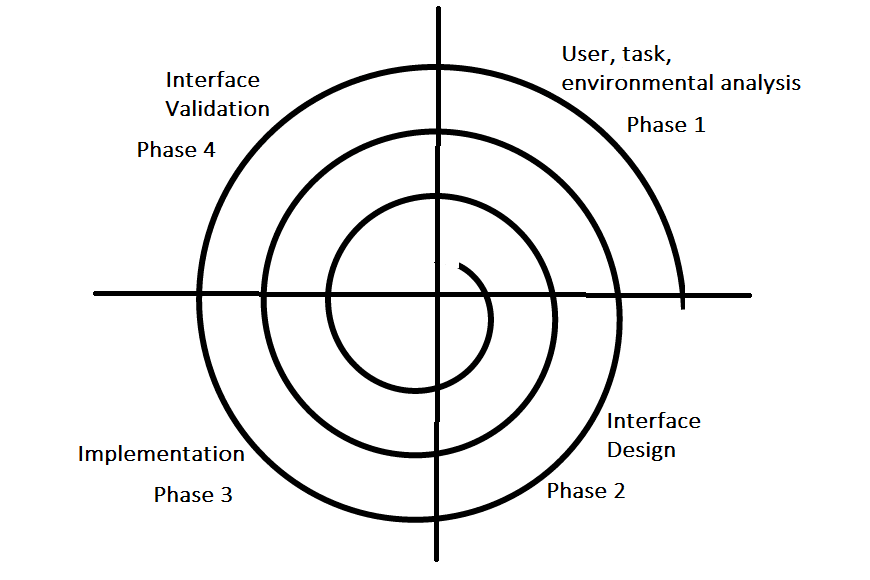
\includegraphics[scale=0.3]{Graphics/espiral}
\caption{Proceso de diseño de interfaz de usuario}
\label{fig:espiral}
\end{figure}

\begin{enumerate}
\item Análisis: El análisis de la interfaz de usuario se centra en el usuario, la tarea, el contenido y el entorno de trabajo que interactúan con el sistema. Inicialmente, el enfoque se basa en el perfil de los usuarios que interactuarán con el sistema, es decir, la comprensión, la habilidad y el conocimiento, el tipo de usuario, etc., según el perfil del usuario, los usuarios se dividen en categorías. De cada categoría se recopilan requisitos. Basado en los requisitos, el desarrollador comprende cómo desarrollar la interfaz. Una vez recopilados todos los requisitos, se realiza un análisis detallado. En la parte de análisis se identifican, describen y elaboran las tareas que realiza el usuario para establecer los objetivos del sistema. El análisis del entorno del usuario se centra en el entorno físico de trabajo.
\item Diseño de la interfaz: el objetivo de esta fase es definir el conjunto de objetos y acciones de la interfaz, es decir, los mecanismos de control que permiten al usuario realizar las tareas deseadas. Indicar cómo estos mecanismos de control afectan al sistema. Especificar la secuencia de acciones de tareas y subtareas, también denominada escenario de usuario. Indicar el estado del sistema cuando el usuario realiza una determinada tarea. Siempre seguir las tres reglas de oro establecidas por Theo Mandel. Los problemas de diseño como el tiempo de respuesta, la estructura de comando y acción, el manejo de errores y las funciones de ayuda se consideran a medida que se refina el modelo de diseño. Esta fase sirve como base para la fase de implementación.
\item Construcción e implementación de la interfaz: La actividad de implementación comienza con la creación de un prototipo (modelo) que permite evaluar escenarios de uso. A medida que continúa el proceso de diseño iterativo, se puede utilizar un conjunto de herramientas de interfaz de usuario que permite la creación de ventanas, menús, interacción de dispositivos, mensajes de error, comandos y muchos otros elementos de un entorno interactivo para completar la construcción de una interfaz.
\item Validación de la interfaz: esta fase se centra en probar la interfaz. La interfaz debería ser tal que debería poder realizar tareas correctamente y debería poder manejar una variedad de tareas. Debe cumplir con todos los requisitos del usuario. Debe ser fácil de usar y fácil de aprender. Los usuarios deben aceptar la interfaz como útil en su trabajo.
\end{enumerate}

Las pruebas determinan la efectividad de una aplicación de interfaz de usuario que debe probarse y expone qué tan fácil o difícil es usar la interfaz de usuario para la audiencia más amplia posible. Los dos principales tipos de pruebas son los siguientes:

\begin{enumerate}
\item Pruebas de usabilidad: evalúan un producto estudiando cómo los usuarios reales realmente usan el sistema. Proporciona una recuperación significativa solo cuando está bien integrado en todo el ciclo de vida del proyecto.
\item Pruebas de accesibilidad: acceden a la aplicación de prueba con tecnologías accesibles y herramientas de prueba automatizadas.
\end{enumerate}

La usabilidad como disciplina constituye un factor determinante de la calidad, cuyo reto es entender cómo los usuarios ven la aplicación web. Por otro lado, la accesibilidad es el grado con que una aplicación web puede ser usada, visitada o accedida por todas las personas independientemente de sus capacidades físicos o técnicas, tema que toma gran importancia para las personas que poseen alguna discapacidad. Ambas disciplinas se encuentran estrechamente relacionadas.

\section{Usabilidad}

En los últimos años, el desarrollo de sistemas interactivos usables y útiles a la vez ha cobrado vital importancia [\cite{1,32}]. Las interfaces de usuario juegan un papel clave en el desarrollo de estos sistemas dado que son las encargadas de  permitir el acceso a los mismos. La usabilidad es un factor clave para el desarrollo de las UI. La usabilidad ha sido definida por la ISO como el grado con que un producto o sistema puede ser usado por usuarios específicos para alcanzar objetivos específicos con efectividad, eficiencia y satisfacción en un contexto de uso dado [\cite{33}]. La dificultad o facilidad que experimenten los usuarios al interactuar con las aplicaciones determinará su éxito o fracaso [\cite{34}]. 

Es importante darse cuenta de que la usabilidad no es una propiedad única y unidimensional de una interfaz de usuario. La usabilidad tiene múltiples componentes y se asocia tradicionalmente con estos cinco atributos [\cite{36}]:

\begin{itemize}
\item Facilidad de aprendizaje: el sistema debe ser fácil de aprender para que el usuario pueda comenzar a trabajar rápidamente con el sistema.
\item Eficiencia: El sistema debe ser eficiente de usar, de modo que una vez que el usuario haya aprendido el sistema, sea posible un alto nivel de productividad.
\item Memorización: el sistema debe ser fácil de recordar, de modo que el usuario ocasional pueda volver al sistema después de un período de no haberlo utilizado, sin tener que aprender todo de nuevo.
\item Errores: El sistema debe tener una tasa de error baja, para que los usuarios cometan pocos errores durante el uso del sistema, y para que si cometen errores, puedan recuperarse fácilmente de ellos. Además, no deben ocurrir errores catastróficos.
\item Satisfacción: El sistema debe ser agradable de usar, de modo que los usuarios estén subjetivamente satisfechos al utilizarlo; les gusta.
\end{itemize}

La usabilidad normalmente se mide haciendo que una cantidad de usuarios de prueba (seleccionados para ser lo más representativos posible de los usuarios previstos) usen el sistema para realizar un conjunto de tareas preespecificado, aunque también se puede medir haciendo que los usuarios reales en el campo realicen las tareas que están haciendo de todos modos. En cualquier caso, un punto importante es que la usabilidad se mide en relación con ciertos usuarios y ciertas tareas.

La usabilidad tiene gran importancia, algunos de sus beneficios son:

\begin{itemize}
\item Una reducción de los costes de producción: los costes y tiempos de desarrollo totales pueden ser reducidos evitando el sobrediseño y reduciendo el número de cambios posteriores requeridos en el producto.
\item Reducción de los costes de mantenimiento y apoyo: los sistemas que son fáciles de usar requieren menos entrenamiento, menos soporte para el usuario y menos mantenimiento.
\item Reducción de los costes de uso: los sistemas que mejor se ajustan a las necesidades del usuario mejoran la productividad y la calidad de las acciones y las decisiones. Los sistemas más fáciles de utilizar reducen el esfuerzo (estrés) y permiten a los trabajadores manejar una variedad más amplia de tareas. Los sistemas difíciles de usar disminuyen la salud, bienestar y motivación y pueden incrementar el absentismo. Tales sistemas suponen pérdidas en los tiempos de uso y no son explotados en su totalidad en la medida en que el usuario pierde interés en el uso de las características avanzadas del sistema, que en algunos casos podrían no utilizarse nunca.
\item Mejora en la calidad del producto: el diseño centrado en el usuario resulta en productos de mayor calidad de uso, más competitivos en un mercado que demanda productos de fácil uso.
\end{itemize}

\section{Accesibilidad}

En la sociedad de la información, las personas acceden a servicios y productos a través de interfaces de usuario. Sin embargo, no todas las personas pueden acceder a ellos, debido a que existen barreras de accesibilidad. Ya no es el caso de que las personas con discapacidad sean los únicos usuarios afectados por las barreras de accesibilidad. De hecho, hoy en día[\cite{39}], numerosos usuarios experimentan problemas a la hora de utilizar la Web, los teléfonos móviles, etc., debido a diferentes tipos de discapacidades, limitaciones funcionales, limitaciones tecnológicas o factores ambientales.

%Para abordar el acceso en este mundo ubicuo, debemos comenzar a pensar en la accesibilidad ubicua y, para algunos, en las interfaces de usuario conectables. La capacidad de "invocar" cualquier tecnología de asistencia o características especiales que se necesiten directamente desde la red para usar en cualquier pantalla que esté cerca, puede ser el medio de acceso más efectivo. Esto es particularmente cierto para las personas que no pueden pagar sus propias tecnologías de la información modernas, sino que confían en las tecnologías que encuentran en los entornos en los que se mueven. Esta capacidad de tener funciones de acceso integradas directamente en la infraestructura que todos usan puede ayudar a nivelar el juego. y, de hecho, significaría que las personas con discapacidad podrían acceder y utilizar las mismas tecnologías principales en los mismos entornos junto con todos los demás.

%La accesibilidad se ha convertido en un tema candente en el diseño web, a pesar de que siempre ha sido parte de la visión original. En un sentido amplio, la accesibilidad simplemente significa garantizar que se pueda acceder a una página determinada en la Web. La accesibilidad no tiene que ver con la discapacidad; más bien, se trata de que las personas accedan a la información compartida que la visión de la Web ha puesto de manifiesto.

%También se ha dicho mucho sobre cómo la accesibilidad se relaciona con los estándares web y viceversa. Siendo realistas, la accesibilidad se basa en aspectos de los estándares web relacionados, pero de hecho se ha convertido en una ciencia, un arte y una práctica propia. Es una especialidad profunda y muy problemática, ya que lo que podría hacer que una página fuera accesible para una persona posiblemente podría volverla inaccesible para otra.

%En informática, la accesibilidad incluye ayudas como las tipografías de alto contraste o gran tamaño, magnificadores de pantalla, lectores y revisores de pantalla, programas de reconocimiento de voz, teclados adaptados, y otros dispositivos apuntadores y de entrada de información.

La accesibilidad aplicada al contenido de Internet se denomina accesibilidad Web. En la Web, el W3C ha desarrollado directrices o pautas específicas para permitir y asegurar este tipo de accesiblidad. El grupo de trabajo dentro del W3C encargado de promoverla es el WAI (\textit{Web Accessibility Initiative}), elaborando para ello unas Pautas de Accesibilidad al contenido Web 1.0, WCAG [\cite{42}].

%Para algunas personas con discapacidades más graves o múltiples, es posible que se necesite una tecnología de interfaz especial que no podría proporcionarse de manera ubicua. Por ejemplo, las personas sordas o ciegas pueden necesitar una pantalla táctil personal. Las personas con discapacidades físicas graves pueden necesitar un transductor de entrada especializado. La capacidad de utilizar estas interfaces alternativas como extensiones naturales de las características ubicuas e integradas permitirá que estas personas también accedan a la Web ya su información. Y la combinación de estos módulos de interfaz personal con software ubicuo y constantemente actualizado puede permitir que estas interfaces especiales funcionen con más y más nuevos tipos de información a medida que evoluciona, aumentando la vida útil de las interfaces y, por lo tanto, reduciendo el costo.

Si bien el acceso a las personas con discapacidad es el enfoque principal de la accesibilidad Web, también beneficia a las personas sin discapacidad. Por ejemplo, un principio clave de la accesibilidad web es diseñar sitios web que sean flexibles para satisfacer las diferentes necesidades de los usuarios. Esta flexibilidad también aumenta la facilidad de uso general y permite que las personas sin discapacidad utilicen los sitios web de acuerdo con sus preferencias, como usar el navegador que deseen y usar atajos de teclado.

Cuando se desarrolla o rediseña un sitio web, la evaluación de la accesibilidad de forma temprana y a lo largo del desarrollo permite encontrar al principio problemas de accesibilidad, cuando es más fácil resolverlos. Técnicas sencillas, como es cambiar la configuración en un buscador, pueden determinar si una página web cumple algunas de las pautas de accesibilidad. Una evaluación exhaustiva, para determinar el cumplimiento de las pautas, es mucho más compleja. 

Hay herramientas de evaluación que ayudan a realizar evaluaciones de accesibilidad. No obstante, ninguna herramienta en sí misma puede determinar si un sitio cumple o no las pautas de accesibilidad. Para determinar si un sitio web es accesible, es necesaria la evaluación humana [\cite{43}].

La accesibilidad de la información basada en la Web se puede mejorar de dos formas principales: mediante el uso de tecnología de acceso y mediante la adopción de buenas prácticas en el diseño de interfaces. Ambos tienen la misma importancia: la provisión de equipos de asistencia (tecnología adaptativa, habilitadora o de acceso) permitirá que un usuario con discapacidad visual acceda a la información en pantalla que recibe la salida de una manera adecuada a sus necesidades. Sin embargo, además de esto, la información proporcionada en pantalla debe presentarse de forma que pueda ser interpretada por cualquier tipo de tecnología de acceso. Esto es lo que se conoce como “diseño web accesible”, “diseño para todos” o “diseño universal”. La necesidad de un enfoque universal ha sido impulsada por la creciente complejidad del diseño y la entrega de información basada en la Web, pasando de una interfaz predominantemente basada en texto a una interfaz multimedia dinámica que ofrece formas visuales, de audio e interactivas. para acceder y utilizar la información proporcionada [\cite{43}].

%Desde un punto de vista técnico, la accesibilidad web es importante para garantizar la interoperabilidad entre diferentes aplicaciones y permitir que los usuarios accedan a la Web utilizando su formato preferido. Esto podría ser a través de tecnología de asistencia para interactuar directamente con el sitio o para descargar información en un formato alternativo.

%Cualquier prueba de accesibilidad debe verse como un proceso que combina herramientas de software automatizadas con juicio humano. No hay ninguna herramienta que pueda ejecutar en su sitio web (o página web, para el caso) para afirmar que es accesible y/o cumple con las disposiciones de la Sección 508 o las Pautas de accesibilidad al contenido web (WCAG)[\cite{43}].

%La interfaz elegida para casi todos los servicios de bibliotecas digitales es la World Wide Web. Aunque se están produciendo cambios significativos en las tecnologías web, la interfaz gráfica de usuario (GUI) se ha convertido rápidamente en la dominante y es probable que siga siéndolo. Desde una perspectiva de accesibilidad, esto ha permitido al menos que se desarrollen enfoques estándar para tratar de garantizar que todos los usuarios puedan acceder a todos los servicios. El sitio web de la biblioteca proporcionará información sobre los horarios de apertura, los servicios ofrecidos y los datos de contacto. También puede ofrecer acceso al catálogo, revistas en línea, resúmenes y páginas de contenido, además de proporcionar acceso en línea a los detalles del prestatario y servicios de renovación y reserva. La provisión de artículos de revistas de texto completo y el desarrollo de la provisión de libros electrónicos brindarán mayores oportunidades para acceder a los servicios de la biblioteca de forma remota. Esto mejorará aún más con la implementación continua de la legislación de derechos de autor que permite que se produzcan formatos alternativos diseñados para personas con discapacidades visuales o de otro tipo a partir de archivos digitales.

\section{Tecnologías empleadas}

Las herramientas de interfaz de usuario han recibido varios nombres a lo largo de los años, siendo el más popular Sistemas de gestión de interfaz de usuario (UIMS). Sin embargo, muchas personas sienten que el término UIMS debe usarse solo para herramientas que manejan la secuencia de operaciones (lo que sucede después de cada evento del usuario), por lo que otros términos como \textit{Toolkits}, Entornos de desarrollo de interfaz de usuario (\textit{User Interface Development Environments}), Constructores de interfaz (\textit{Interface Builders}) y Marcos de aplicación (\textit{Application Frameworks}) también han sido usados [\cite{31}].

Se han diseñado muchos tipos de herramientas para ayudar a crear software de interfaz de usuario, y estos se pueden clasificar por los estilos de las interfaces que crean y las técnicas utilizadas por el diseñador de la interfaz de usuario para crear el software.

%Se han diseñado muchos tipos de herramientas para ayudar a crear software de interfaz de usuario, y estos se pueden clasificar por los estilos de las interfaces que crean y las técnicas utilizadas por el diseñador de la interfaz de usuario para crear el software. Sin embargo, ahora es imposible discutir todas las herramientas de interfaz de usuario, ya que hay muchas. Por ejemplo, hay más de 100 creadores comerciales de interfaces gráficas de usuario, y cada año se informa sobre muchas herramientas de investigación nuevas en conferencias como el Simposio anual de tecnología y software de interfaz de usuario de ACM (UIST) y la conferencia ACM SIGCHI. Por lo tanto, este documento intenta brindar una descripción general de los enfoques más populares, en lugar de una encuesta exhaustiva [\cite{31}].

% En ciencias de la computación, una biblioteca (o library, en idioma inglés) es un conjunto de subprogramas utilizados para desarrollar software. Las bibliotecas de componentes de interfaz de usuario contienen código y datos, que proporcionan servicios a programas independientes, es decir, pasan a formar parte de estos; permitiendo que el código y los datos se compartan y puedan modificarse de formammodular. Algunos programas ejecutables pueden ser a la vez programas independientes y bibliotecas,npero la mayoría de estas no son ejecutables (3).

%Ejecutables y bibliotecas hacen referencias (llamadas enlaces) entre sí a través de un proceso conocido como enlace, que por lo general es realizado por un software denominado enlazador. La mayoría de los sistemas operativos modernos proporcionan bibliotecas que implementan la mayoría de los servicios del sistema. De esta manera, estos servicios se convierten en una "materia prima" que cualquier aplicación moderna espera que el sistema operativo ofrezca. Como tal, la mayor parte del código utilizado por las aplicaciones modernas se ofrece en estas bibliotecas.

%El mundo de la creación de aplicaciones web ha dado pasos agigantados en las últimas décadas. No hace mucho tiempo, clasificar a un trabajador de TI como "desarrollador web" significaba que tenía experiencia en lenguaje de marcado de hipertexto (HTML), hojas de estilo en cascada (CSS) y conocimientos mínimos de JavaScript (JS). Se usó HTML para formatear el contenido y las palabras del sitio web, se usó CSS para hacer que el sitio se viera atractivo con una variedad de colores y diseños y, finalmente, se usó JavaScript para agregar animaciones elegantes en toda la aplicación. Aunque las aplicaciones frontend modernas todavía usan estas tres tecnologías de desarrollo (o lenguajes de desarrollo) en su núcleo, ya no es aceptable simplemente tener un conocimiento "mínimo" de JS. Las demandas de páginas web complejas y completas aumentaron en la esfera del desarrollo frontend, y esto naturalmente resultó en un JavaScript más complejo.

%A medida que aumentaba la complejidad de la cantidad de JavaScript que se incorporaba a la aplicación web, también aumentaba el concepto de lo que significa ser una aplicación web. Los desarrolladores no solo tenían que dar cuenta de la parte frontal de un sitio web, ahora también existe una sección de backend que necesita atención. Aunque no existe una definición de diccionario, una explicación común de lo que se considera backend versus frontend es que “el desarrollo [frontend] es una programación que se enfoca en los elementos visuales de un sitio web o aplicación con los que un usuario interactuará (el lado del cliente). El desarrollo [back-end] se enfoca en el lado de un sitio web que los usuarios no pueden ver (el lado del servidor)”. (Goins, 2020). Cuando las partes de frontend y backend de un sitio web se combinan en una aplicación, la aplicación se considera una aplicación de "pila completa". Las aplicaciones Full Stack requieren más esfuerzo de mantenimiento que las aplicaciones frontend simples, y ahí es donde entran en juego los marcos.

%Desde la aparición de la famosa arquitectura cliente-servidor en la década de los 60, siendo IBM/OS 360 el precursor en esta arquitectura, la misma conforme han pasado los años, se ha desarrollado de manera exponencial, hoy en día los términos front end y back end hacen alusión a esta técnica; siendo el front end el estandarte del cliente mientras que el back end es el estandarte del servidor.

%La construcción de un front end es una tarea delicada dentro de la creación de un proyecto, debido a que no solo puede regirse a los gustos del desarrollador o del cliente, sino también debe regirse a las capacidades técnicas que nos brindan determinadas herramientas de desarrollo. Una página web tradicional se diferencia a una aplicación web porque, la primera hace referencia a una página con información estática no susceptible a la manipulación, mientras, que la aplicación es aquella que se ejecuta en la web así manipulando, procesando presentando y transmitiendo los resultados de manera online, siendo el usuario el que se relaciona directamente con el resultado de ese proceso, denominado producto de información.

Los \textit{frameworks frontends} ofrecen la base para crear y, además, permiten ser flexible respecto a los diseños a implementar. Actualmente, se encuentran una multitud de diferentes \textit{frameworks} con los cuales se pueden realizar un mismo trabajo, aunque cada uno dispone de una curva de aprendizaje distinta, así como sus peculiaridades, conformando diferentes ventajas y desventajas [\cite{48,53}].

En la figura que se muestra a continuación, se puede visualizar cuáles han sido los \textit{frameworks} más de ``moda'' y cómo han ido variando en los últimos años, según el porcentaje de preguntas obtenidas en el famoso dominio ``Stack Overflow''.

\begin{figure}[htp]
\centering
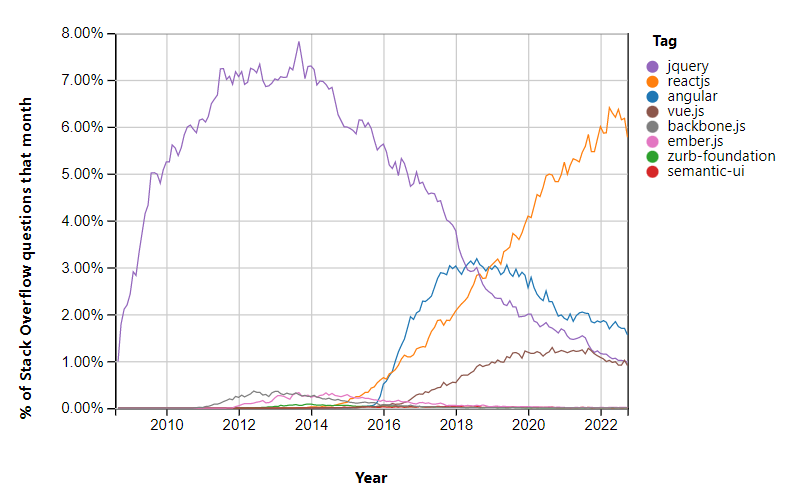
\includegraphics[scale=0.9]{Graphics/stackoverflow}
\caption{Porcentaje de preguntas en Stack Overflow sobre distintos \textit{frameworks}. Fuente:[\cite{50}]}
\label{fig:stackoverflow}
\end{figure}

En la figura anterior, también se observa que, actualmente, los frameworks más usados son React y Angular, sin embargo, Vue se va haciendo un hueco cada vez mayor en la comunidad de interfaces de usuario.

%El desarrollo frontend es un campo que cambia constantemente debido a la gran cantidad de herramientas que se ponen a disposición cada año. Uno de los marcos más populares que se utilizan para crear una experiencia de usuario fluida es el marco Vue. Partiendo del conocido Angular.js, Vue.js es un proyecto independiente de código abierto que está dejando su huella en la comunidad de interfaces de usuario. %51

\subsection{Vue}
%Vue es un framework progresivo JavaScript, esto quiere decir que las principales características, como pueden ser el renderizado y el sistema de componentes, se encuentran ubicadas en una pequeña biblioteca, aunque es posible añadir todas las funcionalidades que se vayan requiriendo según el tipo de proyecto. Algunas de esas características que pueden ser añadidas, que ya traen de partida otros frameworks, son el routing, en el lado del cliente, o manejo de estados mediante vuex o pinia. Esta filosofía permite incluir en la aplicación solo las funcionalidades requeridas.
Vue es un \textit{framework} de JavaScript para construir interfaces de usuario. Se basa en HTML, CSS y JavaScript estándar y proporciona un modelo de programación declarativo y basado en componentes que lo ayuda a desarrollar interfaces de usuario de manera eficiente, ya sean simples o complejas [\cite{47}].

%El principal objetivo que nos encontramos con Vue es la creación de interfaces de usuarios, es por eso por lo que la palabra Vue, es como se denomina a la capa de presentación del modelo MVC (modelo-vista-controlador). El enfoque MVC redujo el uso de recursos de memoria, el tiempo de navegación y la recuperación de datos mediante la reutilización de componentes y la carga parcial del sitio web, obteniendo flexibilidad y comunicación con otras aplicaciones y hardware

Vue es conocido por tener una curva de aprendizaje poco profunda y una implementación progresiva [\cite{49}]. El término framework progresivo por sí mismo es una ventaja, Vue es un \textit{framework} que se puede a aplicar a cualquier proyecto que tenga implementado otras tecnología. También se puede crear proyectos desde cero pensados en escalar su tamaño y sus funcionalidades, como es el caso del sistema que ocupa el tema de esta tesis.

%El manejo de sus componentes, archivos y ficheros, la organización que brinda el entorno de desarrollo para el desarrollador front-end es muy limpia y clara.

El DOM Virtual representa la gran ventaja que Vue cuenta por encima de otro framework [\cite{52}], esta tecnología traída desde React, permite a Vue, no perder tiempo ni rendimiento al cargar todo el árbol de nodos o componentes.

Una de las características, que hace muy cómodo el desarrollo en este \textit{framework}, es que permite dividir las aplicaciones en distintos bloques funcionales independientes llamados componentes, esto se suele denominar arquitectura de componentes. Esta arquitectura permite generar aplicaciones a base de la reutilización de estos componentes, evitando tener código redundante. Además las considerables bibliotecas de componentes de Vue facilitan la reutilización de código, mejoran la productividad del desarrollador y aceleran el proceso de desarrollo.

%Otra de las virtudes de Vue es la capacidad de que las interfaces sean reactivas. Esto significa que se actualiza el HTML y CSS cuando se modifican datos de la aplicación sin que los programadores tengan que realizar una propagación de los cambios de datos de manera manual.

%En cambio, VueJS utiliza el patron Model-View-ViewModel (MVVM) o tambien conocido como Model-View-Whatever. Este patron tiene como objetivo simplificar el desarrollo y el mantenimiento del software. MVVM se divide en 3 partes. Modelo, igual que en otros patrones, representa la capa de datos, contiene la informacion pero nunca la modifica. Vista, su funcion es la de mostrar la informaci ´ on que los usuarios veran. El punto de conexi ´ on entre los 3 componentes comentados anteriormente es el ViewModel o modelo de la vista, donde su funcion es obtener los datos y manipularlos para que se muestren de la forma deseada en la vista. Normalmente hay una ViewModel para cada vista.[7]

%El enfoque Modelo Vista-Controlador redujo el uso de recursos de memoria, el tiempo de navegación y la recuperación de datos mediante la reutilización de componentes y la carga parcial del sitio web, obteniendo flexibilidad y comunicación con otras aplicaciones y hardware

%Las características más importantes de VueJs son:
%• Es un framework progresivo, ya que se puede aplicar a una parte especifica de un aplicativo web
%• Es accesible y escalable
%• Es reactivo, lo que quiere decir tolerante a los fallos
%• Es versátil, ya que el núcleo de VueJs es ligero, y ocupa poco espacio de memoria (74 KB)
%• Tiene una comunidad de programadores que se incrementa, quienes están constantemente mejorando el núcleo.

%Axios es una herramienta familiar en Vue.js porque se usa para mostrar solicitudes AJAX al servicio web. Axios permite crear solicitudes a una URL GET, PUT, POST, DELETE como una API simple, y además posee una biblioteca basada en promesas para recuperar la respuesta con la devolución de llamada [\cite{46}]. 

La herramienta Axios permite crear solicitudes a una URL GET, PUT, POST, DELETE como una API simple, y además posee una biblioteca basada en promesas para recuperar la respuesta con la devolución de llamada. Axios es una herramienta familiar en Vue.js [\cite{46}] lo cual es beneficioso para nuestro sistema que necesita establecer comunicación con el \textit{backend} a través del servicio REST API.
%En la devolución de llamada, se devuelven los datos para la instancia del componente. (Gore 2017).

Vue también brinda una capa de enrutamiento que permite organizar mediante el uso de url, las vistas o componentes se mostrarán en la página, esta capa es fundamental dentro de la seguridad de una aplicación web, ya que permite detener accesos indebidos a vistas destinadas a otros tipos de roles.
Esta capa es muy útil para nuestro sistema que cuenta con distintos roles y permisos para acceder a los datos.

%Aunque Vue está dirigido a aplicaciones de una sola página , también brinda una capa de enrutamiento que permite de mejor manera organizar el contenido en la aplicación. La capa de enrutamiento es aquella, que nos permite organizar mediante el uso de url’s, las vistas o componentes que mostraremos en la página, esta capa es fundamental dentro de la seguridad de una aplicación web, ya que permite detener accesos indebidos a vistas destinadas a otros tipos de roles. peryu

La administración de estado en concepto amplio se refiere a la manera en la que Vue manipula los datos entre componentes estén o no relacionados, generando una especie de almacén donde los componentes podrán acceder para recuperar sus datos [\cite{52}]. 
%La administración de estado en conceptos amplio se refiere a la manera en la que VueJS manipulara los datos entre componentes estén o no relacionados, generando una especie de almacén donde los componentes podrán acceder para recuperar sus datos con respecto a la definición [Vuex busca ayudarnos a lograr una mejor administración del estado imponiendo una tienda centralizada, esencialmente a una sola fuente] (Halliday, 2018).peryu

La persistencia de datos es otra ventaja importante que implementa Vue. Esta función permite que los datos se guarden en el navegador, para que puedan ser usados por los componentes dentro de la vista creada por Vue [\cite{50}]. Añadir la persistencia de datos a nuestro sistema permite optimizar el flujo de las peticiones entre \textit{backend} y \textit{frontend}.

%La persistencia de datos es una pieza clave dentro del rendimiento y la filosofía de desarrollar en VueJS, cualquier aplicación web debe contar con un sistema persistente de datos, para optimizar los flujos de peticiones entre back-end y front-end. peryu

%Gracias a varias características útiles de Vue.js, es una opción preferida para crear muchos sitios web y aplicaciones. Sin embargo, Vue.js se concentra más en la lógica de la aplicación que en su apariencia. Muchos creadores crearon varios marcos de interfaz de usuario de interfaz de usuario para que Vue.js diseñe la interfaz de usuario de manera profesional. Vuetify es uno de estos marcos. Fue creado por John Leider, quien ha trabajado en la comunidad de Vue desde 2014 y cuenta con el respaldo de un vibrante foro de la comunidad de Discord. Vuetify confía en que funcionará en todos los navegadores, incluidos los navegadores antiguos como IE11 y Safari 9 con el requisito de babel-polyfill. Vuetify proporciona varios

%Fortalezas y ventajas de VueJS como herramienta de desarrollo.

%• El termino framework progresivo por sí mismo es una ventaja, VueJS es un framework que se puede a aplicar a cualquier proyecto que tenga implementado otras tecnología, tan solo con importar VueJS traído desde un CDN (Content Delivery Network). También se puede crear proyectos desde cero pensados en escalar su tamaño y sus funcionalidades.

%• No crear nuevas cosas, aunque contradictoriamente el no haber creado nada nuevo, le da una ventaja, puesto que VUEJS logro tomar lo bueno de todas las tecnologías creadas y las transformo en una herramienta más fácil de usar, sin perder robustez.
%• Su entorno para el desarrollo de front-end genera un buen ambiente, sus herramientas son intuitivas y fáciles de usar, obviamente para personas familiarizadas con los conocimientos en el desarrollo front-end.
%• Su reactividad es un framework que se orienta a brindarle a su front–end información constantemente actualizada, bajo esta orientación los desarrolladores solo deben preocuparse en su propósito, generar un buen diseño e una buena interacción con el usuario.
%• El manejo de sus componentes, archivos y ficheros, la organización que brinda el entorno de desarrollo para el desarrollador front-end es muy limpia y clara.
%• Su comunidad, al tener una curva de aprendizaje baja, muchos desarrolladores se suman día a día a esta comunidad desarrollando nuevas herramientas y resolviendo problemas.

%Debilidades y desventajas de VueJS como herramienta de desarrollo.
%
%• La robustez de sus herramientas no oficiales, al ser un framework libre y escalado por la comunidad, sus herramientas complementarias no reciben apoyo de los grandes exponentes en el desarrollo web.
%• El statu quo en el desarrollo de front-end, esta desventaja aunque ajena a la propia herramienta, pone a VueJS fuera de la mira de grandes empresas o proyectos, los desarrolladores tiene una tendencia de mantener las mismas tecnologías.

%En septiembre de 2020, la primera versión de Vue.js, Vue 2, se actualizó a Vue 3. La actualización tuvo un mejor rendimiento general debido a una disminución en el tamaño del código, así como un nuevo formato para manipular la información de la aplicación.

%En cuanto al nivel de presentación se ha elegido el lenguaje Typescript junto con la versión 3 del framework VueJS. VueJS es un framework de javascript que nos permite crear interfaces de manera rápida, escalable y sencilla. Permite desarrollar software de distintas formas, una de ellas es la reactiva, renderizando vistas cuando ocurre un evento, como su rival React. El núcleo de VueJS es muy ligero, convirtiéndolo en un framework muy versátil [35]. En este proyecto se ha trabajado mediante API de composición, lanzada en la versión 3 de Vue, que se centra en funciones de composición, las cuales favorecen la reusabilidad de la lógica entre componentes. Una pieza muy importante es el uso de setup, donde se escribe el código de inicialización del componente a modo de constructor y a su vez se declara el estado reactivo exponiéndolo a la plantilla [36, 14].

Con todo lo expuesto anteriormente, se puede comprobar que Vue es una tecnología que trae beneficios en función de las propiedades deseadas para la interfaz a implementar, pues es liviano, curva de aprendizaje relativamente plana y relativamente fácil de integrar con tecnologías heredadas o una aplicación sin un marco específico. Por estas razones fue el marco de trabajo seleccionado para la solución del problema del presente trabajo.

\subsection{Pinia}

%Hoy en día es necesario hacer uso de alguna librería que nos permita gestionar el estado, almacén de datos compartido por los componentes de la aplicación. La versión 3 de VueJS nos facilita Pinia, librería que gestiona el estado haciendo uso de un store [37]. Un store es un almacén centralizado para mantener los datos que están disponibles, se ha generado uno por cada módulo favoreciendo a la división del código.

Pinia es un nuevo sistema de gestión de estado para Vue [\cite{57}]. Esta es una gran herramienta para cuando se desea compartir datos entre componentes en la aplicación. Una de las razones para usar una herramienta como Pinia (o Vuex para el caso) es que lanzar eventos y escuchar estos eventos en la aplicación puede volverse bastante desordenado y desestructurado. Los sistemas de gestión de estados como Pinia (Vuex, Redux, etc.) pueden ayudar a solucionar esto.

Una gran ventaja de Pinia es su diseño modular, a diferencia de Vuex que proporciona solo una tienda la cual puede tener múltiples módulos dentro de ella, en Pinia se pueden crear varias tiendas que pueden ser importadas directamente a los componentes donde son necesarias[\cite{57}]. Esto permite una mejor división del código y simplifica el desarrollo lo cual es beneficioso para el sistema del presente trabajo.

Pinia tiene soporte integrado para Typescript [\cite{57}], lo cual permite integrar de forma nativa definiciones de tipo dentro de las acciones de Pinia y obtener documentación automática sobre los argumentos que toman las acciones. Además, la seguridad de tipos agrega muchos beneficios a nuestra aplicación, como la prevención de posibles errores de tiempo de ejecución.

Por las razones anteriormente expresadas fue seleccionado Pinia como el sistema de gestión de estados de la aplicación Vue que sera implementada para dar solución al problema de este trabajo.

%Pinia tiene una API más simple que Vuex: La API de Pinia es más simple e intuitiva que Vuex.

%Pinia tiene un diseño modular: Vuex le proporciona una sola tienda que puede tener múltiples módulos dentro de ella. Mientras que en Pinia, puede crear varias tiendas que se pueden importar a componentes directamente donde se necesitan. Esto permite a los empaquetadores dividir mejor el código y proporciona mejores inferencias de TypeScript.
%Tener varias tiendas en lugar de una sola también simplifica el desarrollo, ya que solo se deben usar los métodos de Pinia Store (o módulo) cada vez, en lugar de toda la tienda en Vuex.

%Pinia tiene soporte integrado para Typescript: Lograr que Vuex admitiera tipos siempre había sido una experiencia dolorosa para los desarrolladores de Vue.js. Pinia es una biblioteca de administración de estado completamente tipada que elimina este problema. La seguridad de tipos agrega muchos beneficios a su aplicación, como la prevención de posibles errores de tiempo de ejecución, pero incluso si no está desarrollando su aplicación en TypeScript, obtendrá otros grandes beneficios, gracias a la experiencia de desarrollador rediseñada de Pinia, como la finalización automática. y autosugestión.
%La compatibilidad con TypeScript de Pinia significa que puede hacer cosas como configurar una interfaz para su estado, integrar de forma nativa definiciones de tipo dentro de las acciones de Pinia y obtener documentación automática sobre los argumentos que toman las acciones, completa con autosugerencia y finalización.

%Por estas razones se seleccionó Pinia como el sistema de gestión de estados de la aplicación Vue.js que se implementará para dar solución al problema de este trabajo.

%Pinia se utiliza para guardar el estado de los componentes. Cada vez que se deben enviar datos a la base de datos, se lleva a cabo un determinado procedimiento. Primero, los datos se almacenan temporalmente dentro de la tienda responsable de Pinia y desde dentro de la tienda se activa una llamada API a través de las denominadas acciones. Cada vez que se utiliza Pinia se pueden crear muchas tiendas (Pinia 2022).

\subsection{Typescript}

TypeScript (TS) es un lenguaje de programación desarrollado por Microsoft. TypeScript (TS) es un lenguaje de programación construido a un nivel superior de JavaScript (JS), porque dota al lenguaje de varias características adicionales como el sistema de tipos, el cual nos permite escribir código con menos errores, más sencillo, coherente y fácil de probar [\cite{58, 59}]. 

Los lenguajes de programación tipificados estáticamente están mejor documentados porque el tipado estático en sí mismo actúa como una documentación [\cite{58,60,61}].Esto es una ventaja porque brinda mayor facilidad para otras personas trabajar con nuestro sistema, el cual requiere de posteriores cambios o arreglos a medida que su uso aumente. 

La compatibilidad con TypeScript de Pinia y Vue fueron un factor decisivo para la elección de este lenguaje, además de los ya mencionados beneficios que trae consigo su empleo.
%Esto quiere decir que TypeScript dota al lenguaje de varias características adicionales que hacen que podamos escribir código con menos errores, más sencillo, coherente y fácil de probar, en definitiva, más limpio y sólido [\cite{58, 59}].


%TypeScript agrega escritura estática a JavaScript. [\cite{58, 59}]

%Se informó que los lenguajes de programación tipificados estáticamente están mejor documentados porque el tipado estático en sí mismo actúa como una documentación.[\cite{58}]

%En septiembre del 2020 se liberó lo que conocemos como Vue 3. Todas las novedades de esta nueva versión han relanzado el framework como uno de los más provechosos, obteniendo los desarrolladores una mayor agilidad en su uso. En esta versión todo el framework ha sido implementado bajo TypeScript, el cual ahora se incorpora por defecto en Vue. Esto facilita la reutilización de código y una detección temprana de errores.

%TypeScript (TS) es un lenguaje de programación construido a un nivel superior de JavaScript (JS). Esto quiere decir que TypeScript dota al lenguaje de varias características adicionales que hacen que podamos escribir código con menos errores, más sencillo, coherente y fácil de probar, en definitiva, más limpio y sólido. Algunas ventajas que presenta este lenguaje son las siguientes:

%• Permite usar tipos: esto trae varias ventajas, permite detectar algunos errores en tiempo de diseño sin llegar a la ejecución como pasa con JavaScript, es más fácil entender el código de un vistazo, si se trabaja con algun editor que admita TypeScript se puede detectar errores mientras escribe el código.
%• Es un lenguaje Orientado a Objetos y se pueden usar las características de este: herencia, interfaces, errores tipográficos genéricos, lo que permite un código más ordenado y limpio.
%• Al ser un superconjunto de JavaScript, amplía todas sus funcionalidades, por lo que es compatible con las bibliotecas de JavaScript existentes.

%TypeScript (TS) es un lenguaje increíblemente bien elaborado que respeta y amplía sus raíces de JavaScript. El sistema de tipos parece más expresivo y menos rígido que el de los lenguajes más estáticos y tipificados léxicamente como C$\#$ o Java. Es posible codificar tipos complejos, incluso recursivos, en TypeScript, y se ha demostrado que la sintaxis de definición de tipo es en sí misma Turing-completa. Por estas razones este lenguaje fue seleccionado para la solución del problema de este trabajo.

%Los tipos TS, como cualquier lenguaje escrito, dejan claras sus intenciones, lo que hace que sea mucho más fácil para otras personas trabajar con su código.

\section{REST API}

%La arquitectura orientada a servicios (SOA) se usa generalmente al desarrollar soluciones de software empresarial. Esto brinda flexibilidad para desarrollar diferentes módulos comerciales como servicios allí al brindar escalabilidad y confiabilidad. Entonces la aplicación se acopla débilmente. SOAP y REST son dos enfoques famosos de los servicios web. SOAP (Protocolo simple de acceso a objetos) es un protocolo, mientras que REST (Transferencia de estado representacional) es un estilo arquitectónico en el que se accede a los servicios en forma de Recursos y, en general, se implementan a través de comunicaciones web a través del protocolo HTTP estándar. Los lenguajes de modelado se utilizan para expresar conocimiento/información sobre el sistema que vamos a desarrollar. Para el servicio REST Varios lenguajes/marcos de modelado están presentes en los mundos de la API REST. RAML, Swagger y API Blueprint ahora se usan ampliamente en el desarrollo de API REST.

REST significa transferencia de estado representacional. Este término fue acuñado por primera vez por Roy Fielding[\cite{62}]. REST se refiere al estilo arquitectónico. El estilo arquitectónico REST describe seis restricciones. Estas restricciones, aplicadas a la arquitectura, fueron comunicadas originalmente por Roy Fielding en su tesis doctoral y definen la base del estilo \textit{RESTful}. 

Las restricciones impuestas por la arquitectura REST [\cite{56,62}] son las siguientes:
\begin{itemize}
\item Interfaz uniforme
\item Sin estado
\item Almacenable en caché
\item Cliente-servidor
\item Sistema en capas
\item Código bajo demanda
\end{itemize}

Una REST API describe un conjunto de recursos y un conjunto de operaciones que se pueden llamar en esos recursos [\cite{56}]. La comunicación de la interfaz de usuario de nuestro sistema con el backend se establece mediante un servicio REST API.

%FS 2022-BA-EP-Wisotzki

%Aunque no hubo regulaciones estrictas sobre las tecnologías utilizadas, se sugirió enfáticamente trabajar con tecnologías ya presentes dentro del departamento y el equipo asesor. Además, el cliente también tenía que estar familiarizado con el desarrollo, lo que limitaba significativamente el número de opciones.

%Uno de los aspectos más importantes para la usabilidad de cualquier servicio es la interfaz entre el usuario y el programa. Nuestro objetivo era crear una experiencia de usuario lo más intuitiva posible. Además, debe ser muy simple y eficiente para realizar cualquier tarea, lo que significa que se debe encontrar un equilibrio entre un diseño limpio y ordenado y una accesibilidad de unos pocos clics para todas las funciones.
%
%Para lograr el mejor resultado en este sentido, la interfaz de usuario está inspirada en el TMT existente, así como en OSMCha. Esto asegura que los operadores que ya están familiarizados con cualquiera de los dos no necesitan acostumbrarse a un nuevo diseño y pueden comenzar a trabajar de inmediato. Por supuesto, el diseño se perfeccionó aún más para proporcionar un diseño elegante pero sencillo.

%La simplicidad es clave para alcanzar los objetivos anteriores. Esto se refleja en la interfaz. Los colores se mantienen modestos y están inspirados en el SRZ. A través de su contraste, las partes importantes son fáciles de detectar cuando se resaltan. Un ejemplo es el conjunto de cambios seleccionado, que claramente se destaca de la lista, sin ser demasiado intrusivo. Siempre se muestra la lista completa de conjuntos de cambios, ya que es la parte clave de la aplicación (para dispositivos móviles con pantallas más pequeñas se puede ocultar) e importante para que el usuario vea la lista actual de un vistazo, independientemente de la página actual. Con las páginas se separan las funciones lógicas, lo que mantiene la interfaz enfocada. Todavía hay una conexión sobre el área de conjunto de cambios común, por lo que el usuario siempre sabe lo que está pasando.
%
%Debido a la estructura simple, usamos íconos para marcar la mayoría de los campos y botones. Esto evita distracciones innecesarias a través del texto y lo hace más fácil para las personas que quizás no hablen el idioma. En conjunto, la interfaz debe ser intuitiva para una amplia gama de usuarios. El diseño también es receptivo para adaptarse a una amplia gama de pantallas.
%Para crear unas interfaces más profesionales de forma ágil, se ha utilizado Tailwind, framework basado en clases que se pueden aplicar con facilidad en el código HTML, optimizando el peso del código CSS. Tailwind es una herramienta muy potente a la hora de crear interfaces, esta se apoya en PostCSS para alcanzar un flujo de desarrollo avanzado y optimizado. Gracias a PostCSS se limpian todas las clases que no se están haciendo uso, manteniendo solamente las que se ha utilizado en el proyecto [38]
%
%La siguiente ilustración muestra el conjunto de APIs que compone el nivel de negocio. La tecnología que ofrece la herramienta Swagger nos permite visualizar y probar estas APIs desde el navegador. Además, aporta la ventaja de documentar y especificar las entradas de una operación definida en cada API [45]. 

\chapter{Propuesta}\label{chapter:proposal}

En el presente capítulo se presenta la solución que se propone para dar respuesta al problema planteado, comentando el abanico de posibilidades que existen para elegir la metodología de desarrollo de \textit{software} más adecuada a nuestro proyecto y sobre el tipo de desarrollo a seguir. Se detallan y justifican los principales actores y se hace una descripción de los casos de usos que incluyen todo lo que el sistema debe hacer. Se describe el diseño arquitectónico, además de los patrones de diseño empleados.

%del diagrama de clases y 
%2.1 Introducción 
%En el presente capítulo se hace una propuesta general del sistema a desarrollar después de haber 
%realizado un estudio detallado de los procesos de negocio que tienen lugar en la Dirección de 
%Investigaciones de la Universidad. Se obtienen el modelo de negocio, se identifican los requerimientos
%funcionales y no funcionales que debe tener el sistema propuesto y el modelo del sistema, como 
%artefactos fundamentales en esta etapa, aplicando la metodología RUP y haciendo uso de la 
%herramienta Visual Paradigm y UML como lenguaje de modelado.
%
%En el presente capítulo se presenta la solución técnica del presente trabajo de diploma, se describe el 
%dominio del problema y conceptos, contiene la descripción de los requerimientos del sistema tanto 
%funcionales como no funcionales, se detallan y justifican los principales actores y se hace una descripción 
%de los casos de usos que incluyen todo lo que el sistema debe hacer.
%
%
%solucion propuesta
%A partir del marco teórico analizado en el capítulo 1, se propone una el desarrollo de una interfaz gráfica 
%de usuario para la visualización de imágenes médicas, basada en los principios básicos de diseño y que 
%incluya dentro de sus requisitos las funcionalidades de algunos de los software para la visualización de 
%imágenes medicas existentes en el mercado.
%La interfaz es la parte del sistema con que el usuario interactúa y la que le facilita el acceso a las 
%funcionalidades del sistema, es por ello que su diseño está orientado hacia los usuarios finales, ya que los 
%mismos no están familiarizados con las ciencias de la computación, por lo que se puede decir que no 
%están interesados en la parte interna de la aplicación (el código), sino en cómo se le muestra y cómo 
%usarla.
%
%En el presente capítulo se presenta la solución que se propone para dar respuesta al problema 
%planteado. Se describen los requisitos funcionales y no funcionales con los que debe cumplir la biblioteca
%de componentes propuesta y se muestra una vista general de la misma.
%Además se muestran detalladamente los elementos utilizados en el proceso de desarrollo de cada uno 
%de los componentes de la solución. Se realiza una descripción detallada de la arquitectura, por la cual se 
%rige el desarrollo de la biblioteca de componentes haciendo énfasis en los puntos cruciales de la misma.
%Además se explican los patrones empleados y se realiza una descripción de los diferentes tipos de clases 
%que son implementadas.
%
%Se definen los requisitos funcionales 
%y no funcionales, además de sus descripciones. Se describe el diseño arquitectónico, además, del 
%diagrama de clases y los patrones de diseño empleados. Se realiza una breve descripción de los 
%componentes que integran la biblioteca de interfaz gráfica de usuario y se define el diagrama de 
%componentes para apoyar la implementación.

\section{Metodología de desarrollo de software adoptada}
Las metodologías son un conjunto de procedimientos, técnicas, herramientas y ayudas a la documentación para el desarrollo de software [\cite{91}]. Guían el proceso de desarrollo de software, e imponen una disciplina sobre el desarrollo del mismo con el fin de hacerlo más predecible y eficiente.

Existen en el mundo diferentes metodologías para llevar a cabo el desarrollo de software. Agrupadas en las conocidas metodologías pesadas o tradicionales y las metodologías ágiles [\cite{92}].

\begin{itemize}
\item Metodología Tradicional: impone una disciplina de trabajo sobre el proceso de desarrollo del \textit{software}, con el fin de conseguir un sistema más eficiente. Se centra especialmente en el control del proceso, mediante una rigurosa definición de roles, actividades, artefactos, herramientas y notaciones para el modelado y documentación detallada.
\item Metodología Ágil: permite adaptar la forma de trabajo a las condiciones del proyecto, consiguiendo flexibilidad e inmediatez en la respuesta para adaptar el proyecto y su desarrollo a las circunstancias específicas del entorno.
\end{itemize}

%Al crear cualquier tipo de software, uno tiene que pasar por algún tipo de proceso de desarrollo del sistema. Este es el proceso de definición, diseño, implementación y prueba del software.[29] Este proceso a menudo también se denomina ciclo de vida de desarrollo de software (SDLC) y se puede clasificar en muchos modelos o metodologías diferentes en función de cómo se estructura el flujo de trabajo del proceso de desarrollo.[30]

%Los modelos o metodologías de desarrollo de software se pueden categorizar por cuán formal y cuán secuencial es el proceso de desarrollo. Formal aquí se refiere a la cantidad de aportes que tiene el cliente durante el proceso de desarrollo, lo informal implica aportes y comunicaciones frecuentes, y lo formal implica aportes solo al comienzo del proceso. Cuán secuencial es un modelo describe si es iterativo o lineal, o en otras palabras cuán flexible es. Un modelo que es altamente secuencial está rígidamente planificado y cada parte del proceso de desarrollo se realiza en un orden específico. Esto hace que el proceso sea más fácil de planificar, pero también hace que la contabilidad de los cambios en medio del proceso sea mucho más difícil.
%
%Dos de los modelos más famosos son el modelo Waterfall y el modelo Scrum. El modelo Waterfall es una forma más antigua de desarrollar software que se puede categorizar como formal y secuencial. Scrum es un modelo más moderno y está en el lado opuesto del espectro, siendo informal e iterativo. Los modelos como Scrum y Kanban a menudo se denominan modelos ágiles.
%
%Más hacia el medio, puede encontrar modelos moderados como los modelos Iterativo e iIncremental. Estos modelos son relativamente incrementales y flexibles, pero menos informales que Scrum o Kanban. El modelo Incremental se divide en iteraciones, donde cada iteración agrega nuevos módulos de software. Estas iteraciones pueden ejecutarse secuencialmente o en paralelo. El modelo iterativo es más flexible, con un enfoque en el desarrollo de iteraciones que se basan en el anterior, lo que en muchos casos puede permitir un poco más de información del cliente durante el proceso.

%Una metodología de desarrollo de software es un enfoque estructurado que incluye modelos de sistemas, 
%notaciones, reglas, sugerencias de diseño y guías de procesos. Las metodologías han evolucionado de 
%manera significativa en las últimas décadas, tanto así, que pueden permitir el éxito o el fracaso de muchos 
%de los sistemas desarrollados para distintas áreas
%
%Dentro de las metodologías de desarrollo de software se encuentran:

%\subsection{RUP}
%
%RUP (\textit{Rational Unified Proces}s) es una metodología tradicional de desarrollo de software basada en la generación de documentación exhaustiva y seguimiento estricto del plan de proyecto. Es útil cuando el proyecto no es cambiante y donde los requisitos, coste y tiempo son conocidos de una manera precisa. RUP hace uso de diagramas UML \nomenclature[UML]{\textbf{UML}}{Es un lenguaje de modelado de software}, dirigido principalmente por casos de uso. Además, RUP es iterativo e incremental, con incrementos de larga duración[\cite{93}].
%
%Las fases del proceso son [\cite{92}]:
%\begin{itemize}
%\item Inicio: Da comienzo el proyecto y se acuerda el alcance de este con los clientes, se identifican los posibles riesgos que pueden aparecer y se elabora un plan de negocio para determinar los recursos.
%\item Elaboración: Se construyen las bases para la construcción de la arquitectura del sistema, mediante diagramas de casos de uso.
%\item Construcción: Esta fase trata de implementar las distintas funcionalidades del proyecto, realizar las pruebas y observar las evaluaciones de los clientes.
%\item Transición: El objetivo de esta fase es garantizar que los requisitos definidos anteriormente han sido cumplidos. Cuando los stakeholders están satisfechos debido a que se han alcanzado los objetivos definidos en la primera fase. Finaliza la fase de transición con el lanzamiento de la aplicación.
%\end{itemize}

%\subsection{XP}
%La metodología XP (\textit{eXtreme Programming}), es una metodología ágil enfocada en equipos de trabajo pequeños, con requerimientos imprecisos y cambiantes [\cite{93}]. XP se puede separar en distintas fases [\cite{92}]:
%\begin{itemize}
%\item Exploración: El cliente expone lo que necesita mediante ``historias de usuario'', requisitos escritos en una o dos frases haciendo uso de un lenguaje común por el cliente. Los desarrolladores hacen una primera estimación de tiempo de cada ''historia de usuario''.
%\item Planificación: El cliente y los desarrolladores agrupan las historias de usuario por entregas, después el cliente las ordenará según sus prioridades.
%\item Desarrollo: Las historias de usuario son llevadas a cabo por los desarrolladores, generando un entregable funcional de cada una. El cliente participa activamente durante esta fase, aportando a los desarrolladores los datos necesarios sobre las historias.
%\item Puesta en producción: En esta fase el cliente decide si la aplicación se pone en producción o faltan entregables.
%\end{itemize}
%
%XP sigue un conjunto de reglas y prácticas, a continuación, se mostrarán las más 
%destacadas [\cite{92}]:
%\begin{itemize}
%\item Programación en pares: XP propone que se programe en pares, dos personas trabajando en el mismo ordenador. Esto minimiza los errores, logrando mejores diseños y obteniendo un código de mejor calidad que cuando se desarrolla individualmente.
%\item Programación dirigida por pruebas (\textit{Test Driven Development}): XP propone un modelo en el que primero se escriben las pruebas y después el desarrollo.
%\item Pruebas de aceptación: El cliente debe especificar distintos escenarios para comprobar que una historia ha sido desarrollada correctamente. Una historia no ha finalizado hasta que pase correctamente todas las pruebas de aceptación.
%\end{itemize}

Tras revisar el abanico de posibilidades metodológicas, y dadas las características del proyecto, del equipo de desarrollo y el poco tiempo disponible, se ha decidido adaptar la metodología Scrum.

%\subsection{SCRUM}
Scrum es una metodología ágil donde se fomenta el trabajo en equipo y entregas continuas con el objetivo de ser altamente productivos [\cite{92}]. Esta metodología incluye distintos roles:
\begin{itemize}
\item \textit{Product Owner}: Representa la voz del cliente, deben de entender las necesidades de estos y encargarse de comunicar el objetivo del proyecto, negociar con el equipo de desarrollo las tareas que realizarán y además dar una opinión acerca de los entregables en cada iteración.
\item \textit{Scrum Master}: Es el encargado del cumplimiento de las reglas de la metodología Scrum, ayudando y fomentando el trabajo en equipo. El \textit{Scrum Master} programa y dirige las reuniones del equipo, asegurando que se cumplen las reglas de estas. Por último, elimina cualquier bloqueo o impedimento que pueda tener el equipo.
\item Equipo de desarrollo: Es el encargado de desarrollar las tareas que se encuentran programadas en el sprint, realizar las estimaciones de tiempo de estas, negociar con el \textit{product owner}, y completar las entregas del producto.
\end{itemize}

%\begin{figure}[htbp]
%\centering
%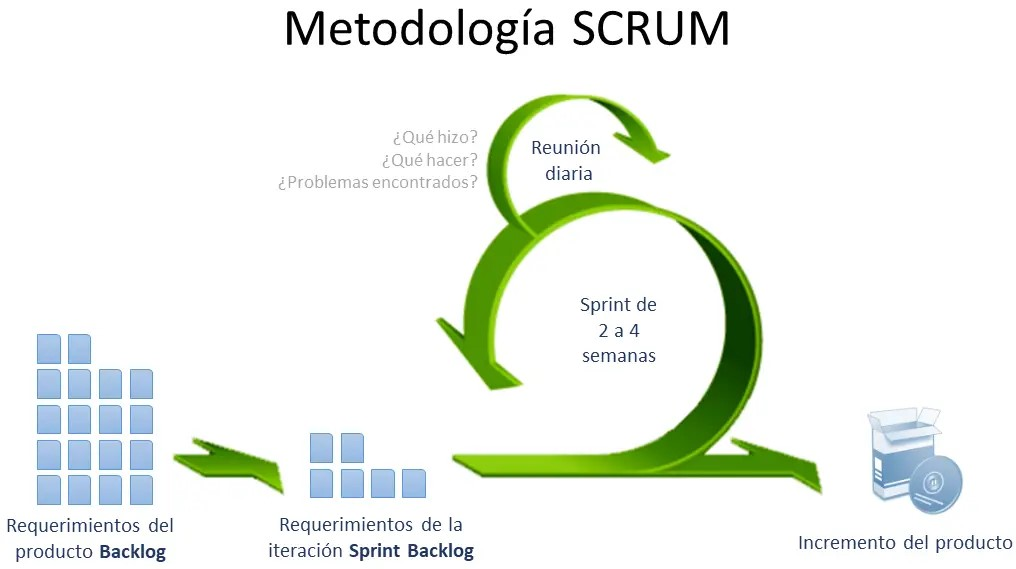
\includegraphics[scale=0.3]{Graphics/SCRUM}
%\caption{Metodología SCRUM [\cite{94}].}
%\label{fig:SCRUM}
%\end{figure}
%
%La Figura \ref{fig:SCRUM} muestra los fundamentos de Scrum. 

Este tipo de metodología trata de realizar entregas del producto final, fijadas en un acuerdo entre el equipo de desarrollo y el \textit{product owner}, para conseguir un resultado completo con cada iteración. Normalmente las iteraciones son de 2 semanas, aunque puede haber equipos que prefieren 3 o 4 semanas.

El \textit{backlog} es un almacén en el cual se encuentran las tareas a realizar, ordenadas por prioridad [\cite{93}]. El equipo de desarrollo es el encargado de añadir y realizar las estimaciones de las tareas, siendo el \textit{product owner} el responsable de priorizar estas. Una vez las tareas se encuentran priorizadas de mayor a menor importancia, según la capacidad del equipo de desarrollo, estos proceden a crear el \textit{sprint}. El \textit{sprint} es el período de tiempo determinado para realizar el trabajo acordado para alcanzar los objetivos propuestos. Es muy importante tener bien definida la tarea, junto con las pruebas de aceptación y una estimación en horas o puntos.

Antes de comenzar un \textit{sprint}, se realiza la reunión llamada \textit{sprint planning}, para seleccionar y comunicar qué tareas es capaz de realizar el equipo, las cuales son seleccionadas del inicio del \textit{backlog}. Una vez finalizado el \textit{sprint} el \textit{product owner} realiza una revisión del trabajo entregado por el equipo de desarrollo y una reunión de retrospectiva en la cual todos los integrantes dejan sus impresiones con el objetivo de mejorar como equipo.

%\item A partir de un identificador, conocer los títulos que posee la persona asociada al identificador.
%\item Autenticar usuarios.
%\item Dado una institución y un rango de fecha listar los diplomas emitidos cumpliendo con la parametrización establecida.
%\item Dado una institución, tipo de diploma, disciplina (carrera / facultad) y un rango de fecha listar los diplomas emitidos cumpliendo con la parametrización establecida.
%\item Dado una institución, disciplina (carrera / facultad) y un rango de fecha listar los diplomas revocados y sus motivos.
%\item Añadir diploma al sistema.
%\item Revocar diploma, pues un título en determinadas situaciones puede ser revocado.

%Tras revisar el abanico de posibilidades metodológicas, y dadas las características del proyecto y del equipo de desarrollo, se ha decidido adaptar el modelo Iterativo a las necesidades del proyecto. Se utilizaron también algunos aspectos del desarrollo ágil, específicamente de la metodología SCRUM, como trabajar en iteraciones y tener alguna parte del sistema funcionando después de cada iteración, para que esto pudiera ser presentado y discutido con el cliente. Esto también ayudó a lograr un proceso de desarrollo más fluido y educativo.

%a las necesidades del proyecto. Siendo el equipo solamente una persona (el autor de 
%este trabajo), no existe ningún rol, pero se mantiene la creación y el mantenimiento del 
%backlog, siguiendo una organización de sprints, permitiendo generar gráficas y ver el 
%estado de trabajo. Si el equipo aumentara en un futuro, se comenzaría a hacer uso de
%los roles definidos en la metodología

%En este proyecto se utilizó un proceso de desarrollo iterativo. Se utilizaron algunos aspectos del desarrollo ágil, como trabajar en iteraciones y tener alguna parte del sistema funcionando después de cada iteración, para que esto pudiera ser presentado y discutido con el cliente. Esto también ayudó a lograr un proceso de desarrollo más fluido y educativo.

%La mayor parte del trabajo del proyecto se realizó en línea. Esto se debió a varias razones, por ejemplo, el hecho de que todos usaban principalmente computadoras de escritorio para el trabajo y se habían acostumbrado a trabajar desde casa durante el covid 19, y las oficinas del cliente estaban a más de una hora de viaje. Los repositorios Git proporcionados por el cliente y la aplicación Telegram sirvieron como plataforma para la cooperación.

\section{Análisis del sistema}
Teniendo en cuenta la propuesta planteada en el capítulo anterior y la metodología de desarrollo adoptada, a continuación se desarrollará el análisis de los principales elementos del sistema. 
%%\subsection{Requerimientos del sistema}
%El Glosario Estándar IEEE de Terminología de Ingeniería de Software define un requisito como condición o capacidad que necesita un usuario para resolver un problema o lograr un objetivo [\cite{95}]. Los requisitos se pueden clasificar en: funcionales y no funcionales.
%
%\subsection{Requisitos funcionales}
%Los requisitos funcionales son capacidades o condiciones que el sistema debe cumplir [\cite{91}]. Su meta principal es identificar y documentar las acciones que en realidad debe ejecutar el sistema para que cumpla con los objetivos planteados al inicio del presente trabajo de diploma.
%
%De acuerdo con los objetivos propuestos el sistema debe ser capaz de:
%
%\begin{enumerate}
%\item A partir de un identificador, conocer los títulos que posee la persona asociada al identificador.
%\item Autenticar usuarios.
%\item Dado una institución y un rango de fecha listar los diplomas emitidos cumpliendo con la parametrización establecida.
%\item Dado una institución, tipo de diploma, disciplina (carrera / facultad) y un rango de fecha listar los diplomas emitidos cumpliendo con la parametrización establecida.
%\item Dado una institución, disciplina (carrera / facultad) y un rango de fecha listar los diplomas revocados y sus motivos.
%\item Añadir diploma al sistema.
%\item Revocar diploma, pues un título en determinadas situaciones puede ser revocado.
%\end{enumerate}
%
%\subsection{Requisitos no funcionales}
%
%Los requisitos no funcionales son propiedades o cualidades que el producto debe tener [\cite{91}]. Debe pensarse en estas propiedades como las características que hacen al producto atractivo, usable, rápido o confiable.
%
%\begin{enumerate}
%\item Requisitos de interfaz y usabilidad:
%	\begin{itemize}
%	\item Tener una interfaz intuitiva y fácil de usar sin necesidad de explicaciones detalladas.
%	\item Contar con una barra de navegación superior y lateral, siguiendo el patrón de los diseños comunes en las aplicaciones actuales.
%	\item Adaptar el contenido adecuadamente al tamaño de pantalla pertinente, ya sea ordenador o dispositivo móvil.
%	\item Usar una paleta de colores consistente.
%	\item Utilizar botones que expresen su función, ya sea a través del ícono o el texto que lo identifica.
%	\item Asegurar que el usuario final sepa dónde se encuentra dentro del flujo procedural de la aplicación, manteniendo una retroalimentación eficiente y completa con dicho usuario.
%	\end{itemize}
%\item Requisitos operacionales:
%	\begin{itemize}
%	\item Ser una aplicación multiplataforma, funcional tanto en sistemas operativos distintos como en dispositivos de diferentes tamaños.
%	\end{itemize}
%\item Requisitos de seguridad:
%	\begin{itemize}
%	\item Tener en cuenta la información visible de los distintos usuarios.
%	\end{itemize}
%\item Requisitos de mantenibilidad y portabilidad:
%	\begin{itemize}
%	\item Tener en cuenta el uso de tecnologías persistentes y una visión de futuro para implementar actualizaciones sin problema alguno.
%	\end{itemize}
%\item Requisitos de recursos:
%	\begin{itemize}
%	\item Ser una aplicación ligera en cuanto al tamaño necesario de almacenamiento.
%	\end{itemize}
%\item Requisitos de rendimiento:
%	\begin{itemize}
%	\item La herramienta debe ser rápida y el tiempo de respuesta debe ser el mínimo posible, al igual que la velocidad de procesamiento de la información.
%	\end{itemize}
%\item Requisitos de disponibilidad:
%	\begin{itemize}
%	\item La aplicación no debe dejar de funcionar aunque se provoquen fallos.
%	\end{itemize}
%\end{enumerate}

%Requisitos no funcionales de Apariencia o Interfaz Externa.
%El usuario debe tener acceso por varias vías a una determinada funcionalidad.
%El sistema debe contener una interfaz sencilla e intuitiva y sea agradable al usuario.
%La herramienta debe utilizar como idioma principal el español, excepto aquellas palabras técnicas 
%que no puedan ser traducidas.
%Utilizar botones que expresen su función, ya sea a través del ícono o el texto que lo identifica.
%Los colores de la interfaz serán agradables, sin mucho brillo que pueda afectar la vista del usuario 
%que tiene sus ojos concentrados en la lectura. 
%Requisitos de Rendimiento.
%La herramienta debe ser rápida y el tiempo de respuesta debe ser el mínimo posible, al igual que la 
%velocidad de procesamiento de la información.

%Fiabilidad en la aplicación: El usuario debe recibir la información mínima sobre
%errores.
%• Seguridad y protección de datos: La aplicación debe cumplir con la normativa
%vigente.
%• Facilidad de uso: El usuario debe ser capaz de usar la aplicación de forma
%intuitiva.
%• Tiempos de respuesta bajos: El usuario no debe recibir esperas prolongadas.
%• Alto nivel de carga: Capacidad para soportar muchos usuarios en la aplicación al
%mismo tiempo.
%• Disponibilidad: La aplicación no debe dejar de funcionar aunque se provoquen
%fallos.
%• Transparencia de acceso: El usuario no debe saber con cuantas entidades se está
%comunicando el sistema.
%• Portabilidad: La aplicación se debe poder usar en cualquier sistema de escritorio.

\subsection{Actores del sistema}
Los actores representan entidades que interactúan con el sistema, un actor del sistema es aquel que se beneficia de los resultados de las funcionalidades del mismo [\cite{91}]. 

Se definen dos tipos de usuarios principales que pueden interactuar con la plataforma: \textbf{anónimos} y \textbf{gestores}. El usuario \textbf{anónimo} es un \textbf{usuario público} que puede acceder sin registrarse a las funcionalidades públicas del sistema.

Los \textbf{gestores} serán usuarios registrados en un sistema de terceros. Estos usuarios tendrán acceso a una sección de \textit{back office} que le permitirá realizar tareas de gestión en la plataforma. Además, contarán con un rol definido en dicho sistema de terceros cuyo rol viajará en la respuesta de autenticación del mismo al nodo cliente (borde del \textit{backend} de la solución a implementar).

\subsection{Casos de uso del sistema}
La forma en que los actores utilizan el sistema puede ser representada a través de los casos de usos [\cite{91}]. Estos últimos son artefactos narrativos que describen, bajo la forma de acciones y reacciones, el comportamiento del sistema desde el punto de vista del actor.

%Los casos de usos identificados en el presente trabajo son enunciados a continuación:
\begin{figure}[!h]
\centering
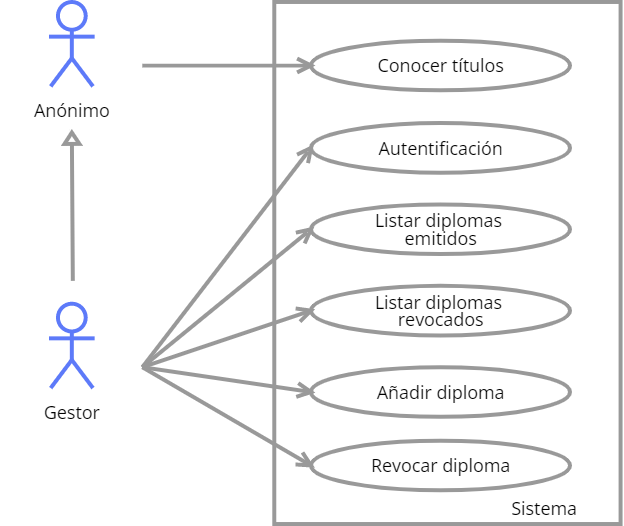
\includegraphics[width=\textwidth]{Graphics/useCasest}
\caption{Diagrama de casos de uso del sistema}
\label{fig:useCases}
\end{figure}

%\subsubsection{Diagrama de casos de uso del sistema}
En la Figura \ref{fig:useCases} se observa el diagrama de casos de uso del sistema a desarrollar. Los diagramas de casos de usos [\cite{91}] son un tipo de diagrama dónde se puede representar el comportamiento esperado del sistema, desde la visión de los usuarios, sin llegar a un alto nivel de especificación acerca de cómo se implementan las acciones. 

%El diagrama de casos de uso del sistema a desarrollar se puede encontrar en la Figura \ref{fig:useCases}.

Los principales elementos que nos encontramos en este tipo de diagramas son:
\begin{itemize}
\item Sistema: Representa con un rectángulo los limites del sistema, los actores se ubican fuera de la figura.
\item Caso de uso: Representado con un óvalo y un texto identificativo, identifican una determinada acción.
\item Actor: Son las entidades externas al sistema que interactúan con el.
\end{itemize}

%\subsubsection{Descripción de los casos de uso del sistema}
A continuación se exponen algunos de los casos de uso de alto nivel, para lograr entender los procesos globales de la aplicación. El resto puede ser encontrado en los anexos \ref{appendix:useCase}.

\begin{table}[!h]
	\begin{center}
		\begin{tabular}{|c|p{10cm}|}
		\hline \textbf{CU1} & Conocer títulos \\ 
		\hline \textbf{Actor} & Anónimo \\ 
		\hline \textbf{Descripción} & El usuario podrá conocer los títulos asociados a una persona al introducir el identificador que representa a la persona.  \\ 
		\hline 
		\end{tabular}
		\caption{Caso de uso: Conocer títulos}
		\label{tab:CU1}
	\end{center}
\end{table}

\begin{table}[!h]
	\begin{center}
		\begin{tabular}{|c|p{10cm}|}
		\hline \textbf{CU2} & Autentificación \\ 
		\hline \textbf{Actor} & Gestor\\ 
		\hline \textbf{Descripción} & El usuario de tipo gestor deberá insertar el nombre de usuario y su contraseña para poder acceder al sistema.\\ 
		\hline 
		\end{tabular}
		\caption{Caso de uso: Autentificación}
		\label{tab:CU2}
	\end{center}
\end{table}

\subsection{Elementos importantes del sistema}
El sistema que se presenta no registrará binarios (copia digital de título, entre otras), sino que los certificados serán representados por propiedades:
\begin{itemize}
\item \textbf{ID}: El identificador de los certificados es con fines de facilitar su búsqueda. No tiene una representación real en un certificado a papel. El campo es generado utilizando la fecha y hora de creación de la credencial. Su estructura es: YYYYMMDDHHMMSS (año, mes, día, hora, minuto y segundo concatenados)
\item \textbf{Certificación}: Título que se le otorga al acreditado.
\item \textbf{Título de oro}: Campo que representa si se alcanzó la distinción.
\item \textbf{Emisor}: Centro que emite el certificado. Ej: Universidad de la Habana.
\item \textbf{Acreditado}: Persona a la que se emite el título.
\item \textbf{Fecha}: Fecha de emisión del documento.
\item \textbf{Creador}: Usuario que creó dicho certificado en la base de datos.
\item \textbf{Secretario, Decano y Rector}: Tres propiedades que guardan los nombres de los funcionarios que validan la Credencial.
\item \textbf{Tomo y folio de facultad y universidad}: Dos propiedades que almacenan Tomo y folio bajo el cual fueron inscritos los documentos tanto en la facultad como en la universidad
\item \textbf{Estado}: Refleja el estado actual del documento.
\item \textbf{Razón de Invalidación}: Refleja, de estar el certificado en estado invalidado, la razón de la decisión.
\end{itemize}

En nuestra aplicación, exisitirán varios roles con distintas funcionalidades. El personal de las instituciones universitarias podrán realizar consultas más especializadas y gestionar los certificados digitales según el rol que posea, para ello necesitarán iniciar sesión con sus credenciales asignadas. Los roles que se manejarán para los usuarios gestores son los siguientes:

\begin{itemize}
\item \textbf{Administrador de Sistemas}: Encargado de manejar los usuarios que participan en el sistema: crearlos, editarlos, eliminarlos o invalidarle sus credenciales.
\item \textbf{Administrador de Certificados}: Usuario que tiene los permisos para gestionar los certificados: crearlos, editarlos, eliminarlos o invalidarlos. Este rol no valida los certificados.
\item \textbf{Secretario General}: Usuario que tiene los permisos para validar certificados recién creados. Puede invalidar los certificados que encuentre inconsistentes.
\item \textbf{Decano de Facultad}: Usuario que tiene los permisos para validar certificados aprobados por el Secretario General. Puede invalidar los certificados que encuentre inconsistentes.
\item \textbf{Rector de Universidad}: Usuario que tiene los permisos para validar certificados aprobados por el decano. Es el último eslabón para hacer un certificado válido. Puede invalidar los certificados que encuentre inconsistentes.
\item \textbf{Inválido}: Usuario al que le fueron retirados sus privilegios por un administrador de sistema.
\end{itemize}

Los certificados pueden tener cinco estados:
\begin{itemize}
\item \textbf{Inválido}: El certificado fue invalidado por un usuario gestor con los permisos adecuados.
\item \textbf{Creado}: El documento fue creado pero no posee ninguna firma de validación.
\item \textbf{Firmado por Secretario}: El documento fue validado por un usuario gestor con rol de `secretario'.
\item \textbf{Firmado por Secretario y Decano}: El documento fue validado por un usuarios gestores con rol `secretario' y `decano'.
\item \textbf{Válido}: El certificado fue validado por usuarios gestores con rol `secretario', `decano' y `rector'.
\end{itemize}
%Para la emisión de los certificados, primeramente el administrador de certificados debe insertar el título. Una vez insertado, el decano debe aprobar o validar este certificado, el cual deberá entonces ser validado por el secretario general para finalmente ser validado por el rector. Para la validez del título debe haber sido validado por las tres últimas entidades mencionadas y siguiendo el orden en el que fueron nombradas.

\subsection{Historias de usuario}
Las historias de usuario se usan, en el contexto de la ingeniería de requisitos ágil, como una herramienta de comunicación que combina las fortalezas de ambos medios: escrito y verbal. Describen, en una o dos frases, una funcionalidad de \textit{software} desde el punto de vista del usuario, con el lenguaje que éste emplearía. Se enfocan en qué necesidades o problemas soluciona lo que se va a construir.

A continuación se exponen algunos de las historias de uso de alto nivel, las demás pueden ser encontradas en los anexos \ref{appendix:useHistory}.

\begin{table}[!h]
	\begin{center}
		\begin{tabular}{|c|p{10cm}|}
		\hline \textbf{H.U-1} & Conocer títulos \\ 
		\hline \textbf{Usuario} & Anónimo\\ 
		\hline \textbf{Descripción} & Como usuario anónimo quiero poder conocer los certificados de una persona para poder observar las habilidades y estudios de esa persona. \\ 
		\hline 
		\end{tabular}
		\caption{Historia de Usuario: Conocer títulos}
		\label{tab:HU1}
	\end{center}
\end{table}

\begin{table}[!h]
	\begin{center}
		\begin{tabular}{|c|p{10cm}|}
		\hline \textbf{H.U-2} & Autentificación \\ 
		\hline \textbf{Usuario} & Gestor \\ 
		\hline \textbf{Descripción} & Como usuario gestor quiero poder autenticarme para poder tener acceso al sistema. \\ 
		\hline 
		\end{tabular}
		\caption{Historia de Usuario: Autentificación}
		\label{tab:HU2}
	\end{center}
\end{table}

\begin{table}[!h]
	\begin{center}
		\begin{tabular}{|c|p{10cm}|}
		\hline \textbf{H.U-3} & Cerrar sesión \\ 
		\hline \textbf{Usuario} & Gestor \\ 
		\hline \textbf{Descripción} & Como usuario gestor quiero poder cerrar la sesión actual para poder salir de forma segura del sistema. \\ 
		\hline 
		\end{tabular}
		\caption{Historia de Usuario: Cerrar sesión}
		\label{tab:HU3}
	\end{center}
\end{table}

\subsection{Planificación de desarrollo}
Siendo el equipo solamente una persona (el autor de este trabajo), no existe ningún rol, pero se mantiene la creación y el mantenimiento del \textit{backlog}, siguiendo una organización de \textit{sprints}, permitiendo tener alguna parte del sistema funcionando después de cada iteración, para que esto pudiera ser presentado y discutido con el cliente. Si el equipo aumentara en un futuro, se comenzaría a hacer uso de los roles definidos en la metodología.

La fecha final del proyecto será acorde a la fecha límite de entrega de la convocatoria ordinaria del Trabajo de Fin de Grado. Por tanto, se ha establecido la duración de los sprints en 2 semanas, teniendo cada uno una carga de 34h aproximadamente por \textit{sprint}. En la tabla \ref{tab:sprints} puede verse una planificación inicial. Esta planificación es susceptible a cambios, así como la fecha de finalización podría ser cambiada.

%        Para la administración de tareas, se ha utilizado la herramienta Jira, creada por la 
%empresa Atlassian, que permite realizar una gestión ágil del proyecto. Jira crea 
%Aplicación web para la gestión de clubes de fútbol
%48
%automáticamente el backlog, que es la lista de trabajo donde se encuentran las tareas 
%encontrándose arriba las más importantes por el propietario del producto [40].
%Dentro de Jira, se puede crear distintos sprints, explicado anteriormente en el punto 
%3.4.1, indicando las fechas y las tareas que existen. Además, permite visualizar los 
%informes del sprint, siendo muy útiles para el equipo de desarrollo y sobre todo para el 
%Scrum máster.
%La plataforma no solo permite la creación y el seguimiento de los sprints, también es 
%posible realizar un seguimiento de los bugs registrados.

\begin{table}[!h]
	\begin{center}
		\begin{tabular}{|p{2cm}|p{3cm}|p{3cm}|p{3.8cm}|}
		\hline \textbf{Sprint} & \textbf{Comienzo} & \textbf{Final} & \textbf{H.U a desarrollar} \\ 
		\hline Sprint 0 & 1/09/2022  & 15/09/2022 & -\\ 
		\hline Sprint 1 & 15/09/2022 & 29/09/2022 & H.U-1\\ 
		\hline Sprint 2 & 29/09/2022 & 13/10/2022 & H.U-2, H.U-3\\ 
		\hline Sprint 3 & 13/10/2022 & 27/10/2022 & H.U-4\\ 
		\hline Sprint 4 & 27/10/2022 & 10/11/2022 & H.U-5, H.U-6, H.U-7\\ 
		\hline Sprint 5 & 10/09/2022 & 24/10/2022 & H.U-8\\ 
		\hline 
		\end{tabular}
		\caption{\textit{Backlog} inicial}
		\label{tab:sprints}
	\end{center}
\end{table}

Debido a la poca experiencia del autor con las tecnologías establecidas por el cliente, se realizará un \textit{sprint} 0 con el objetivo de analizar y aprender estas tecnologías para la correcta realización del proyecto.

\section{Diseño del sistema}
Tras el apartado de análisis, en el que se ha establecido cuales son los elementos que se desean incluir en el sistema, se desarrolla a continuación el apartado, en el que se explica cómo se quieren llevar a cabo los requisitos.

\subsection{Arquitectura del sistema}
La arquitectura de un \textit{software} se encarga de entender cómo debe organizarse el sistema y cómo tiene que diseñarse la estructura global del mismo [\cite{91}]. Constituye el enlace crucial entre el diseño y la ingeniería de requisitos, ya que identifica los principales componentes estructurales en un sistema y la relación entre ellos. La salida del proceso de diseño arquitectónico consiste en un modelo arquitectónico que describe la  forma en que se organiza el sistema como un conjunto de componentes en comunicación. La arquitectura de \textit{software} representa un elemento fundamental pues afecta el desempeño del sistema, así como su capacidad de distribución y mantenimiento.

Según [\cite{99}], la arquitectura de un sistema puede basarse en un patrón o un estilo arquitectónico particular. Un patrón arquitectónico es una descripción de una organización del sistema, captan la esencia de una arquitectura usada en diferentes sistemas de \textit{software}.

%Para empezar la sección de diseño, se va a exponer la arquitectura del sistema que se va a
%implementar, destacando dos aspectos relevantes, el patrón de diseño Modelo Vista VistaModelo (MVVM) y la denominada arquitectura backendless

%Para la realización del sistema se apuesta por la división de 3 niveles: presentación, lógica de negocio y persistencia. 
%
%\begin{figure}[htp]
%\centering
%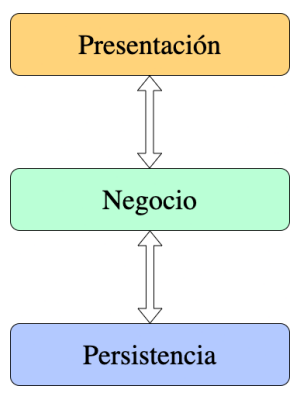
\includegraphics[scale=0.9]{Graphics/levels}
%\caption{Arquitectura del sistema}
%\label{fig:3levels}
%\end{figure}
%
%La arquitectura de tres niveles organiza el sistema en distintos niveles lógicos y físicos. El nivel de presentación, donde se encuentra la interfaz del usuario, en la cual se enfoca el presente trabajo; el nivel de negocio, donde se encuentra toda la lógica para procesar los datos y, por último, el nivel de persistencia, donde se almacenan los datos [\cite{96}]. Cada nivel puede encontrarse en una infraestructura distinta y desacoplado de los demás, por lo que estos niveles pueden escalar y actualizarse según sea necesario. Suele haber una confusión entre nivel y capa. La división en capas es simplemente la división funcional, sin embargo, la división en niveles es una división funcional y de infraestructura. Esto quiere decir que el \textit{software} se ejecuta en distintas máquinas y no en la misma.
%
%El nivel de presentación es la encargada de mostrar al usuario la información, interactuar con él y ajustar estos datos a las especificaciones que son demandadas por la capa de negocio. En el caso de nuestra aplicación este nivel se ejecuta en el navegador web. 
%
%El nivel de negocio es el encargado de facilitar al nivel de presentación los datos necesarios, a la vez que recolecta los datos aportados por este para procesarlos. Este nivel está también conectado con el nivel de persistencia, enviándole peticiones para almacenar o recuperar datos de este [\cite{96}].
%
%El nivel de persistencia es donde residen los datos y generalmente está formada por un gestor encargado de realizar el almacenamiento de datos. Este nivel recibe las peticiones de negocio, quien le dice qué datos necesita o qué datos tiene que almacenar. El nivel de persistencia no se puede comunicar directamente con el nivel de presentación, siempre debe de comunicarse con negocio previamente [\cite{96}]. 
%
%%Vue.js utiliza una arquitectura basada en componentes, separando así grandes trozos de código en componentes más pequeños. Además, en Vue.js, todo es un componente, y cada componente está escrito con HTML, CSS y JavaScript, lo que favorece la legibilidad y la simplicidad.
%%
%%El back-end proporcionará endpoints para el registro y el acceso de un usuario, así
%%como una API CRUD para el manejo de notas (crear, recuperar, actualizar y eliminar);
%%y será el front-end el que haga uso de estos puntos de acceso para darle al usuario un
%%servicio de notas online.
%
%Como mencionamos previamente, el presente trabajo de diploma se enfoca en el desarrollo del nivel de presentación. 

El empleo de Vue para el desarrollo de nuestra solución nos permite dividir la aplicación en distintos bloques funcionales independientes llamados componentes, esto se suele denominar arquitectura de componentes[\cite{50}]. Todos los componentes relacionados entre sí se agrupan y se comunican entre sí para realizar las tareas. Esta arquitectura permite generar aplicaciones a base de la reutilización de estos componentes, evitando tener código redundante.

La arquitectura de nuestra solución es una arquitectura \textit{N-Layer} adaptada a las características del proyecto (ver Figura \ref{fig:spa}). Cuando el usuario accede en el navegador a nuestra aplicación, internamente al componente raíz App.vue se le pasa un componente enrutador, el cual debe hacer uso de las rutas definidas para cargar la vista deseada por el usuario. Las vistas son las diferentes ventanas de la página web (página principal, la lista de usuarios, entre otras), mientras que los componentes son pequeños trozos de código que se repiten en las diferentes vistas (barra de navegación, botones, entre otras). Para trabajar con datos, las vistas invocan a las funciones de Pinia, las cuales se encargan de realizar las peticiones a la API, la cual escucha y responde a las solicitudes de los clientes. Las peticiones a la API se realizan mediante la herramienta Axios, la cual también es la encargada de realizar las acciones necesarias para recopilar los datos y enviar la respuesta de vuelta a Pinia. Cuando Pinia ya ha obtenido la respuesta, este envía los datos a la vista, quien muestra al usuario el contenido de la ruta a la que accedió.


%La arquitectura de este nivel está basada en componentes. Todos los componentes relacionados entre sí se agrupan y se comunican entre sí para realizar las tareas. Por ejemplo, el componente de carga interactúa con el componente de inicio cuando se realiza la carga para actualizar la interfaz de usuario. Toda la funcionalidad se realiza en estructuras de componentes pequeños y estos componentes están diseñados para ser reutilizables.

La arquitectura de nuestra interfaz de usuario también se basa en las arquitecturas cliente-servidor y SPA. Las SPA se caracterizan por cargar todos los recursos de la aplicación web en la consulta inicial, como si se tratara sólo de una página. Los componentes cambian dinámicamente a medida que el usuario va interaccionando con ellos. Esto proporciona una interfaz de usuario más rápida y fluida, ya que todas las representaciones se realizan localmente en el navegador del usuario. La página solicita nueva información del servidor cuando los datos se almacenan o se obtienen del servidor (Ver Figura \ref{fig:spa}).

\begin{figure}[htbp]
\centering
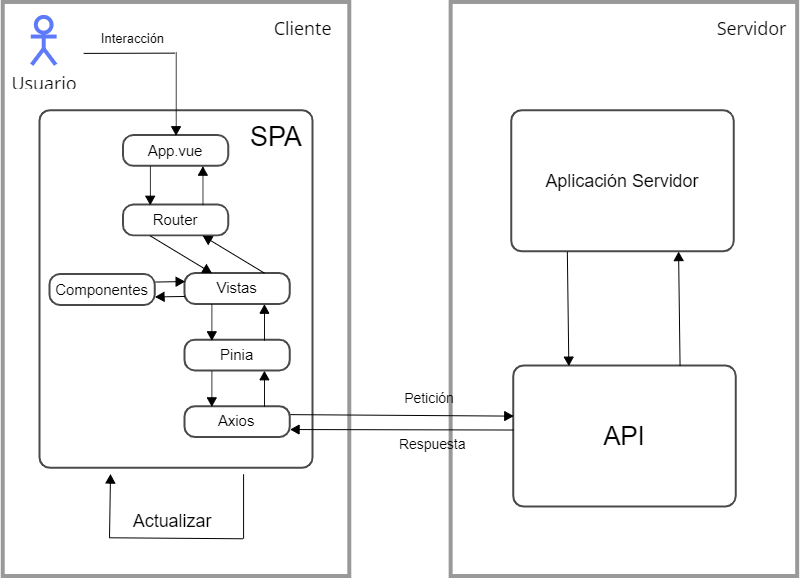
\includegraphics[width=\textwidth]{Graphics/mySPAtt}
\caption{Arquitectura de la solución}
\label{fig:spa}
\end{figure}

\subsection{Patrones de diseño}

La arquitectura es necesaria para comprender el sistema, organizar el desarrollo, fomentar la reutilización y hacer evolucionar el sistema. Para definirla es muy importante tener en cuenta un patrón de diseño o modelo de abstracción que nos sirva para poder estructurar de manera eficaz todos los componentes de la aplicación, tanto la parte de la interfaz (vista), como la de la lógica (controlador) y la del modelo de datos (modelo).

%necesario seleccionar y combinar patrones. Los patrones de diseño constituyen la base para la búsqueda de soluciones a problemas comunes en el desarrollo de software y otros ámbitos referentes al diseño de interacción o interfaces. Un patrón de diseño es una solución a un problema de diseño; facilitan la reusabilidad, extensibilidad y mantenimiento. 

\subsubsection{Patrón MVVM}

El patrón Modelo Vista Vista Modelo o en inglés Model View ViewModel (MVVM) se diferencia del clásico Modelo Vista Controlador (MVC) [\cite{45}]. En el MVC, es el controlador (el componente encargado de toda la lógica de la aplicación que enlaza la vista con el modelo) quien debe actualizar manualmente los cambios producidos en el modelo o en la vista de manera independiente, mientras que en el patrón MVVM, estos cambios se actualizan automáticamente gracias al componente VistaModelo. Es decir, si se produce un cambio en la vista, los datos son actualizados de forma automática en la parte del modelo, y viceversa.

Por ejemplo, el entorno de desarrollo Vue está centrado en el componente Vista-Modelo del patrón MVVM [\cite{49,47}], que se encarga del trabajo realizado por el controlador en el diseño MVC, pero enlazando los datos entre la vista y el modelo de forma reactiva, simple y flexible.

\begin{figure}[htbp]
\centering
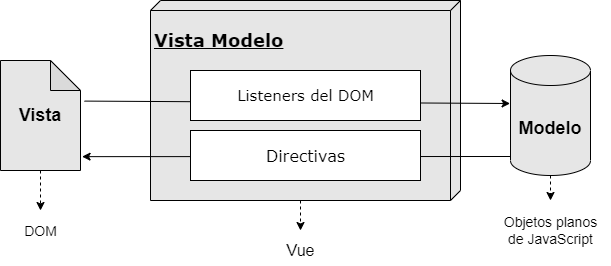
\includegraphics[width=\textwidth]{Graphics/mvvm}
\caption{Patrón de diseño MVVM en Vue [\cite{47}].}
\label{fig:vmmv}
\end{figure}


%Todos estos son marcos que utilizan un patrón de diseño Model-View-Viewmodel (MVVM). Aquí, el modelo representa la lógica comercial de back-end, la vista representa el diseño de la interfaz de usuario y el modelo de vista representa el código intermediario entre los dos, que maneja la lógica de la vista. Ver figura 4.
%
El objetivo principal de una implementación de MVVM es separar la lógica de la interfaz de usuario de la lógica empresarial. Esto nos trae varias ventajas, una de ellas es la separación de preocupaciones. Esto significa que evita el código estrechamente acoplado y resistente al cambio, el cual a menudo puede causar problemas durante el mantenimiento o la actualización. Otra ventaja importante es que permite a un solo desarrollador poder desarrollar y probar una aplicación completa sin tener mucha experiencia con el diseño de UI como es el caso del autor de este proyecto.
%
%Una de las características clave de MVVM Frameworks es el enlace de datos entre los datos de la vista y la lógica del modelo de vista. El enlace de datos es la práctica de vincular un proveedor de datos y un consumidor de datos, y con esto permitir una conexión bidireccional. Esto es muy útil en el contexto del desarrollo de Frontend porque desea vincular la interfaz de usuario a la lógica, pero estos generalmente están en dos idiomas diferentes, por ejemplo, HTML y JavaScript. Al usar el enlace de datos, los elementos de la interfaz de usuario en la vista se pueden cambiar dinámicamente desde la lógica en el modelo de vista.
%
%El patron Modelo Vista Vista Modelo o en inglés Model View ViewModel, es una variación del MVC que está diseñado para plataformas de desarrollo de interfaz de usuario modernas donde la vista es responsabilidad de un diseñador en lugar de un desarrollador. MVVM se basa en un mecanismo general de enlace de datos que facilita el desarrollo de la capa de separación de vista desde el resto del patrón mediante la eliminación de todo el código subyacente de la capa de la vista. 
%
%El modelo, encapsula la lógica de negocio y datos. La lógica empresarial se define como cualquier lógica de aplicación que se ocupa de la recuperación y gestión de datos de la aplicación y de asegurar que las reglas del negocio que garanticen la coherencia de los datos y la validez se cumplan. Para maximizar las oportunidades de reutilización, los modelos no deben contener ningún caso de uso o conducta específica del usuario o lógica de la aplicación. 
%
%La vista, encapsula la interfaz de usuario y la lógica de la interfaz de usuario. Las vistas definen la interfaz de usuario específica para una parte de la aplicación, son normalmente los controles que se han diseñado para funcionar bien cuando se une a un ViewModel.
%
%El viewmodel, encapsula la lógica de presentación y estado. Lógica de presentación se define como la lógica de la aplicación que se ocupa de casos de uso de la aplicación (o casos de usuario, tareas de usuario, flujo de trabajo, etc.) y define el comportamiento lógico y la estructura de la aplicación. Para maximizar las oportunidades de reutilización, el ViewModel no debe tener ninguna referencia a las clases específicas de interfaz de usuario, elementos, controles o comportamiento.
%

%El modo MVVM es el mismo que el modo MVC, el propósito principal es separar la vista (Vista) del modelo (Modelo), hay varias ventajas
%
%Acoplamiento bajo: las vistas pueden ser independientes de los cambios y modificaciones del modelo. Un modelo de vista se puede vincular a diferentes vistas. Cuando la vista cambia, el modelo puede permanecer sin cambios, y cuando el modelo cambia, la vista también puede permanecer sin cambios.
%Reutilizable: puede poner algo de lógica de vista en un modelo de vista y permitir que muchas vistas reutilicen esta lógica de vista.
%Desarrollo independiente: los desarrolladores pueden centrarse en la lógica empresarial y el desarrollo de datos (ViewModel), y los diseñadores pueden centrarse en el diseño de páginas.
%Comprobable: la interfaz siempre ha sido difícil de probar, pero ahora la prueba se puede escribir para ViewModel.

%Modelo: capa de modelo, que representa objetos JavaScript aquí
%Vista: capa de vista, donde DOM (elemento de manipulación HTML) se representa aquí
%ViewModel: middleware que conecta vistas y datos, Vue.js es el implementador de la capa ViewModel en MVVM
%En la arquitectura MVVM, los datos y la vista no pueden comunicarse directamente y solo pueden comunicarse a través de ViewModel, y ViewModel define un observador
%
%ViewModel puede observar cambios de datos y actualizar el contenido correspondiente a la vista
%ViewModel puede monitorear cambios en la vista y notificar cambios en los datos
%En este punto, entendemos que Vue.js es un implementador de MVVM, y su núcleo es implementar el monitoreo DOM y el enlace de datos.

%Entre los elementos de un patrón se encuentran: Nombre (describe el problema de 
%diseño), Problema (describe cuándo aplicar el patrón) y Solución (describe los elementos que 
%componen el diseño, sus relaciones, responsabilidades y colaboración).
%
%En aplicaciones grandes, es posible que necesitemos dividir la aplicación en partes más pequeñas y solo cargar un componente del servidor cuando sea necesario. Para hacerlo más fácil, Vue le permite definir su componente como una función de fábrica que resuelve de forma asíncrona la definición de su componente. Vue solo activará la función de fábrica cuando el componente deba renderizarse y almacenará en caché el resultado para futuros renderizados.

%Los componentes y contenedores no son más que el patrón de diseño Mediator. Donde los componentes serán los que se encargar de pintar, podrán tener lógica de pintado, pero muy poca. Reciben datos y los pintas, nada más. Los contenedores son aquellos que orquestan a los componentes y les pasan los datos. Suelen tener más lógica pero no suelen tener ni estilos visuales ni markup.
%
%Los componentes se comunican con los contenedores mediante eventos, y los contenedores se comunican con los componentes mediante props. Esto hace que los tests sean mucho más fáciles, los componentes estén más desacoplados y si falla algo en cuanto a la orquestación, sabremos que tenemos que mirar el contenedor.
%

%Encapsulación: propone esconder algunos componentes, permitiendo sólo accesos estilizados al 
%objeto. Se hace uso de este patrón en casi todas las clases que componen la solución, permitiendo que 
%estas solo posean como elementos públicos aquellos que son exclusivamente necesarios (24).
%Subclase: propone heredar miembros por defecto de una superclase, seleccionando la implementación 
%correcta a través de resoluciones sobre qué implementación debe ser ejecutada. Se puede encontrar este 
%patrón con más fuerza en las entidades de negocio que por su conceptualización las funciones y la 
%información que almacenan pueden estar diferenciadas en cierta medida (24).
%Fábrica: provee de una interfaz para crear familias de objetos relacionados o dependientes sin 
%especificar los tipos concretos de clases. Su uso se encuentra centrado a la creación de los conectores 
%correspondientes al acceso a datos que se esté utilizando, así como en la obtención de los servicios a 
%utilizar (24).

%Vue: permita que el cliente almacene el estado local de una manera funcional basada en patrones de observadores
%Este patrón de diseño le permite suscribirse y emitir eventos desde componentes de su aplicación.
\subsubsection{Patrones GRASP}
Los patrones GRASP (Patrones Generales de Software para Asignación de Responsabilidades) describen los principios fundamentales de diseño de objetos para la asignación de responsabilidades. Las responsabilidades  están relacionadas con las obligaciones de un objeto en cuanto a su comportamiento [\cite{97}]. Entre los patrones GRASP empleados en la solución encontramos:

\begin{itemize}
\item Bajo Acoplamiento: El acoplamiento es una medida de la fuerza con que una clase está conectada a otras clases, con que las conoce y recurre a ellas. El bajo acoplamiento soporta un diseño de clases más independientes, que reducen el impacto de cambios, y permite que sean más reutilizables.

La arquitectura de software basada en componentes permite un bajo acoplamiento entre sus componentes. Estos pueden ser creados, modificados o eliminados en cualquier momento, lo que proporciona que la dependencia entre ellos sea baja.

\item Alta Cohesión: La cohesión es una medida de la fuerza con la que se relacionan las clases y el grado de focalización de las responsabilidades de un elemento. Cada elemento del diseño debe realizar una labor única dentro del sistema, no desempeñada por el resto de los elementos, y auto-identificable. Una clase con baja cohesión realiza muchas labores no relacionadas o realiza demasiado trabajo.

La arquitectura de software basada en componentes permite la organización del trabajo en cuanto a la estructura del proyecto y la asignación de responsabilidades con una alta cohesión. Cada componente realiza solo las funcionalidades para las cuales fueron creados, colaborando entre ellos para cumplir con el resto de las funcionalidades, generando un bajo acoplamiento y fomentando la reutilización. Esto hace posible que el sistema sea flexible a cambios sustanciales con efecto mínimo
\end{itemize}

\subsubsection{Patrones GoF}
Los patrones GoF (Patrones de la ``pandilla de los cuatros'') son los más utilizados en la implementación de \textit{software} [\cite{97}]. Los patrones GoF utilizados en la propuesta de solución son los siguientes:

\begin{itemize}
\item Singleton (Instancia Única): Su propósito es asegurar que una clase tenga una única instancia y proporcionar un punto de acceso global a dicha instancia.

En la solución se ve presente al instanciar el hilo principal de la aplicación, la clase encargada de la autenticación de usuarios y la clase encargada de la comunicación, garantizando un único punto de acceso y evitando la replicación de hilos y proceso.

\item Observer (Observador): Este patrón define una dependencia de uno-a-muchos entre objetos, de manera que cuando un objeto cambie de estado se notifique y actualicen automáticamente todos los objetos que dependen de él.

Los servicios de gestión de estado de Vue utilizan el patrón de observador, permitiendo al cliente almacenar el estado local de una manera funcional [\cite{52}]. El patrón se utiliza como soporte para que el sistema pueda comunicarse con una API externa accediendo a los datos brindados por el paquete de servicios (Pinia). En esta solución permite mantener consistencia entre objetos relacionados sin aumentar el acoplamiento entre clases.

\end{itemize}
%A continuación se presenta los patrones de diseño GoF que fueron seleccionados para utilizar como 
%parte de la solución:
%Singleton: Su propósito es asegurar que una clase tenga una única instancia y proporcionar un 
%punto de acceso global a dicha instancia en este caso esa función la realiza la clase “MainController”. 
%De esta forma se logra crear una variable global, que hace el objeto accesible y para que sea posible 
%instanciarla sólo una vez. En consecuencia hay un acceso controlado a dicha única instancia, y se 
%gestionan de manera centralizada los recursos utilizados.
%Follwing the singleton pattern, we created a new file in which we created a new instance
%of Axios that could be reused and imported whenever needed
%
%Decorator: Añade capacidad de desplazamiento a una vista. Para este caso facilita los cambios 
%dinámicos en la apariencia de la aplicación cuando se aplica la configuración de alto contraste para 
%mejorar la lectura de los discapacitados visuales. 
%Observer: Se utiliza para definir una dependencia de uno-a-muchos entre objetos, de forma que 
%cuando un objeto cambie de estado se notifique y actualicen automáticamente todos los objetos que 
%dependen de él. En esta solución permite mantener consistencia entre objetos relacionados sin 
%aumentar el acoplamiento entre clases.

%Observer 
%31
%Este patrón define una dependencia de uno-a-muchos entre objetos, de manera que 
%cuando un objeto cambia de estado, todos sus dependientes son notificados y 
%actualizados automáticamente. En la solución se ve presente cuando ocurre cualquier 
%evento que el usuario necesite conocer, automáticamente la consola es notificada para 
%que actualice su estado, también se puede presenciar en el módulo de creación de salvas 
%periódicas, cuando cambia el estado de la configuración, automáticamente es enviada la 
%notificación para realizar o no la creación de las salvas.
%Singleton
%Es un patrón creacional cuyo principal objetivo es garantizar que una clase solo tenga
%una única instancia, proporcionando un punto de acceso global a la misma. En la solución 
%se ve presente al instanciar el hilo principal de la aplicación, la clase encargada de la 
%autenticación de usuarios y la clase encargada de la comunicación, garantizando un 
%único punto de acceso y evitando la replicación de hilos y proceso

%2.4.1 Patrones GRASP24
%Una de las actividades más complicadas en Orientación de Objetos consiste en elegir las clases 
%adecuadas y decidir como estas clases deben interactuar. 
%Experto: La responsabilidad de realizar una labor es de la clase que tiene o puede tener los datos 
%involucrados (atributos). Una clase, contiene toda la información necesaria para realizar la labor que tiene 
%encomendada.
%Creador: El patrón Creador guía la asignación de responsabilidades relacionadas con la creación de 
%objetos. El propósito fundamental de este patrón es encontrar la clase responsable de crear una nueva 
%instancia de determinada clase.
%Controlador: Un Controlador es un objeto que se encarga de manejar un evento del sistema. Este no 
%realiza mucho trabajo por sí mismo, sino que delega en otros objetos, coordina y controla el trabajo que se 
%necesita hacer.

%2.4.2 Patrones GoF
%25
%Singleton (Instancia Única): Está diseñado para restringir la creación de objetos pertenecientes a una 
%clase a un único objeto. Asegura que una clase tiene una sola instancia y proporciona un punto de acceso
%global a ella.
%Factory Method (Método de Fabricación): Define una interfaz para crear un objeto dejando a las 
%subclases decidir al tipo específico al que pertenecen.
%Algunas de las ventajas de este patrón son:
%Centralización de la creación de objetos.
%Facilita la escalabilidad del sistema.
%El usuario se abstrae de la instancia a crear.
%Facade (Fachada): Simplifica los accesos a un conjunto de clases relacionadas proporcionando una
%única clase que todos utilizan para comunicarse con dicho conjunto de clases.

%Patrones GRASP5
%(Patrones Generales de Software para Asignación de Responsabilidades):
%Según (Grosso 2011), son patrones basados en la asignación de responsabilidades a objetos. Es una 
%buena práctica para el desarrollo eficaz de la Programación Orientada a Objetos (POO).
%• Experto: consiste en asignar la responsabilidad de realizar una labor a la clase que tiene o puede 
%tener los datos involucrados
%
%Creador: consiste en asignar a una determinada clase B la responsabilidad de crear una instancia 
%de la clase A al ocurrir alguna de las siguientes circunstancias
%
%Bajo acoplamiento: consiste en asignar una responsabilidad a una clase de manera que el 
%acoplamiento permanezca bajo. Una clase con bajo (o débil) acoplamiento no depende de muchas 
%otras clases
%
%La arquitectura de software basada en componentes permite un bajo acoplamiento entre sus 
%componentes. Estos pueden ser creados, modificados o eliminados en cualquier momento, lo que 
%proporciona que la dependencia entre ellos sea baja.
%• Alta cohesión: consiste en asignar una responsabilidad de manera que la cohesión permanezca 
%alta. La cohesión es una medida de la fuerza con la que se relacionan las responsabilidades de un 
%elemento.
%La arquitectura de software basada en componentes permite la organización del trabajo en cuanto a la 
%estructura del proyecto y la asignación de responsabilidades con una alta cohesión. Cada componente 
%realiza solo las funcionalidades para las cuales fueron creados, colaborando entre ellos para cumplir con 
%el resto de las funcionalidades, generando un bajo acoplamiento y fomentando la reutilización. Esto hace 
%posible que el sistema sea flexible a cambios sustanciales con efecto mínimo

%Patrones GoF6
%(Patrones de la “pandilla de los cuatros”):
%Los patrones GoF son los más utilizados en la implementación de algún software, se clasifican por su 
%propósito en creacionales, estructurales y de composición, mientras que respecto a su ámbito se clasifican 
%en clases y objetos (Gamma et al. 1997). Los patrones GoF utilizados en la propuesta de solución son los 
%siguientes:
%• Decorator (Decorador): proporciona metadatos adicionales a las clases que determinan cómo el 
%componente se debe procesar, instanciar y usar en tiempo de ejecución.
%
%• Observer (Observador): se utiliza como soporte para que el sistema pueda comunicarse con una 
%API7
%(Interfaz de Programación de Aplicaciones) externa accediendo a los datos brindados por el 
%Paquete de Servicios

%• Singleton (Instancia única): se encarga de asegurar que una clase tenga una sola instancia y 
%que proporcione un punto de acceso global a ella. El uso de este patrón es necesario cuando 
%existen clases que tienen que gestionar de manera centralizada un recurso.
%\subsection{Principios de diseño}
%El diseño de la interfaz orienta al usuario respecto al lugar donde se encuentre, mediante la barra de título. 
%Los mensajes de ayuda, así como el del botón cerrar provee al usuario de una respuesta inmediata; el
%sistema cuenta con un área de mensaje de estado donde se muestra información sobre la tarea que el 
%usuario está realizando en ese momento. 
%La interfaz propuesta posee una barra de herramienta donde aparecen las funcionalidades más usadas 
%por el usuario; cuenta con un panel de control donde estarán ubicados los diferentes parámetros que se 
%corresponden con la ejecución de las funcionalidades y los elementos incluidos en esta barra de 
%herramientas poseen un tamaño razonable para que no resulte difícil dar clic sobre ellos. Los íconos 
%utilizados para la representación de estas funcionalidades no se utilizan para otra cosa que no sea su 
%finalidad prevista y los colores utilizados en los mismos son de gran contraste entre ellos y respecto al 
%color de fondo. Se le da al usuario la posibilidad de cerrar la aplicación en el momento que así lo desee,mostrándole un mensaje de confirmación de la acción en caso que el usuario no esté seguro del 
%procedimiento.
%La interfaz le da la posibilidad al usuario de acceder a la ayuda del sistema en caso que este se encuentre 
%desorientado. La información se sitúa con sutileza para facilitar la interacción del usuario con la aplicación, 
%con un tamaño de letra para los íconos y menús (MS Shell Dlg 2), tratando de variar al mínimo. Para el 
%color de las letras se utiliza el negro que se distingue sobre el fondo gris y esto le aporta seriedad a las 
%aplicaciones de este tipo. El diseño proporciona una serie de menús desplegables que solo se muestran
%cuando el usuario hace clic en uno de ellos; los mismos están visibles en todo momento y son accesibles
%desde el teclado.

%Un principio de diseño es un conjunto de buenas prácticas para la actividad del diseño, 
%de las cuales se pueden desprender la identificación de piezas en las cuales 
%descomponer el sistema, la asignación de responsabilidades a esas piezas, garantizando 
%la manera en que interactúan unas con otras [38].
%A continuación, se mencionan los principios de diseño utilizados en el desarrollo de la 
%aplicación:
%Single responsibility principle (Principio de única responsabilidad)
%Define que una clase o función de una clase deben tener una única razón para cambiar. 
%Se debe analizar si existe más de una posible razón que puedan generar cambios en 
%una clase o una función, si es así, puede ser que esta se esté dedicando a más de un 
%tipo de responsabilidad, con lo cual, será más probable que cambie a menudo y será 
%potencialmente menos reutilizable. Este principio se utiliza en la solución en general, 
%donde las clases tienen responsabilidad única, por ejemplo, la clase Client tiene la única 
%responsabilidad relacionada con la comunicación con el Servidor

%Ley de Demeter 
%Este principio establece que las operaciones de una clase, solamente deberían efectuar 
%llamadas a objetos que cumplan una de las 4 características siguientes: a sí mismos, a 
%objetos pasados como argumento, a objetos creados por ella y a objetos con los cuales 
%tiene relaciones directas.
%Once and Only Once Rule 
%Este principio establece la no repetición de una misma responsabilidad en más de una 
%clase o módulo, en la medida en que alguna función es repetida en un mayor número de 
%lugares, a la hora de modificar esa función, se pueden quedar varias de las piezas 
%afectadas sin actualizar el cambio. Si por el contrario esa regla o función estuviera 
%implementada en un único lugar, efectuar un cambio en ese único lugar, haría que el 
%cambio quedara integrado al sistema consistentemente.

%\subsection{Diagramas de diseño}

\subsection{Elementos de seguridad}

% ---------------------------------- seguridad
Como habíamos mencionado previamente en la definición de actores del sistema, los gestores son usuarios registrados en un sistema de terceros y además cuentan con un rol definido en dicho sistema de terceros. Nuestra interfaz de usuario debe ser capaz de mostrar visualmente las secciones del \textit{back office} relacionadas a los permisos asociados al rol del usuario autenticado.

%JSON Web Token es una forma alternativa de autorizar usuarios a la forma tradicional de usar sesiones. Tradicionalmente, los identificadores de sesión se almacenan en el servidor y se transmiten a la \textit{cookie} del cliente. Cuando el cliente realiza una solicitud al servidor, la identificación de la sesión del cliente se pasa a través del campo de encabezado en la solicitud HTTP al servidor. Luego, el servidor compara la identificación de la sesión recibida del cliente con la almacenada en el servidor. Si coinciden, la solicitud se resuelve; si no, la solicitud se rechaza.

La autentificación de portador (también llamada autenticación de token) es un esquema de autentificación HTTP que involucra tokens de seguridad llamados \textit{Bearer tokens} [\cite{98}]. El nombre ``Autenticación de portador'' puede entenderse como ``dar acceso al portador de este token''. El \textit{Bearer token} es una cadena críptica, generalmente generada por el servidor en respuesta a una solicitud de inicio de sesión.

Tanto en el servidor, como en el sitio web, nos centraremos en la seguridad. Entre otras cosas: el servidor creará y verificará tokens de identificación (\textit{Bearer token}) para cada usuario, y nuestra interfaz los usará para saber quien está identificado en cada momento y los permisos asociados a ellos; todas las contraseñas de los usuarios se guardarán en formato hash usando la función bcrypt; y, por último, todos los datos recibidos por el servidor se validarán para evitar usos incorrectos.

%JWT opera de una manera diferente. Un token solo se almacena en el lado del cliente de la aplicación, y no en el servidor. En cuanto a la escalabilidad, es mejor usar JWT para autorizar solicitudes, ya que no se almacena en el servidor, por lo tanto, no utiliza la memoria del servidor.

El siguiente diagrama contiene una propuesta de cómo se debe realizar el proceso de autenticación y la interacción de cada parte.

\begin{figure}[!h]
\centering
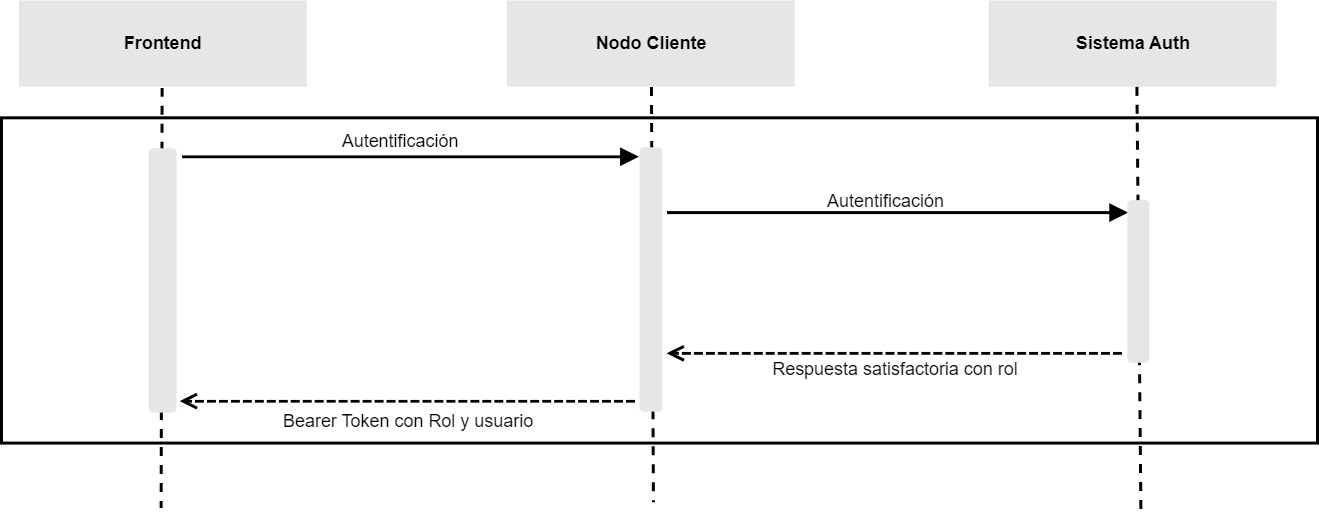
\includegraphics[width=\textwidth]{Graphics/authtt}
\caption{Diagrama de secuencia del proceso de autentificación del sistema.}
\label{fig:autht}
\end{figure}

%
%Se envía un token JWT a través de la solicitud HTTP al servidor. Luego, el servidor decodifica y valida el token. Si se valida el token, se resuelve la solicitud, si no, se rechaza la solicitud. JWT es propuesto como un estándar abierto por IETF y es elegido por muchos como la tecnología de referencia para la autorización.
%JWT hace que la autorización sea fácil e intuitiva

\subsection{Diagrama de despliegue}
Un modelo de despliegue consiste en una representación estructural de la arquitectura del sistema desde el punto de vista de la distribución de los artefactos del software en los destinos de despliegue; definiendo a los artefactos como representaciones de elementos concretos en el mundo físico que son el resultado de un proceso de desarrollo [\cite{91}]. 

\begin{figure}[htbp]
\centering
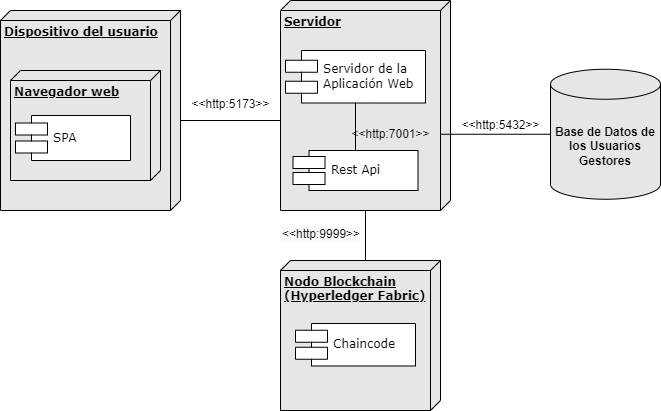
\includegraphics[width=\textwidth]{Graphics/deploy}
\caption{Diagrama de despliegue del sistema.}
\label{fig:deploy}
\end{figure}

%Como ya hemos indicado en el apartado anterior, Vue es el framework elegido para la 
%parte del servidor Web. Este framework se apoya en NodeJs, que es un entorno de 
%ejecución de JavaScript orientado a eventos asíncronos, y que será la base para la 
%construcción del módulo Front-End. A su vez, para la creación de los servicios REST 
%desde el componente de la interfaz web, se utiliza Axios, un cliente HTTP basado en 
%promesas para Javascript.
%Estas llamadas serán recibidas por el Back-End, 

%A continuación, se muestra el diagrama de despliegue 
%propuesto para el Portafirmas Digital. El mismo, muestra la disposición física de los nodos que componen 
%el sistema y el reparto de los componentes en dichos nodos.

\chapter{Detalles de Implementación y Experimentos}\label{chapter:implementation}
La etapa de implementación del \textit{software} es el proceso de convertir una especificación del sistema en un sistema ejecutable. Esta fase comprende la materialización, en forma de código, de todos los artefactos, descripciones y arquitectura propuestos en la etapa de análisis y diseño; con el objetivo de conformar el producto final requerido por el cliente [\cite{91}].

Una vez desarrollado el \textit{software}, el mismo debe ser sometido a una serie de pruebas que muestren que el sistema se ajusta a su especificación y que cumple con las expectativas del usuario. Según [\cite{91}], esta etapa es conocida como la validación e implica una serie de procesos de comprobación, como las inspecciones y revisiones. Por lo que el presente capítulo tiene como objetivo documentar los resultados de las fases de implementación del sistema y de la estrategia de pruebas desarrollada, y validar la solución propuesta.

%El desarrollo de las vistas del nivel de presentación está compuesto por 
%componentes, piezas de código con un comportamiento específico que unidos crean 
%aplicaciones web [46], si estos se abstraen correctamente pueden ser reutilizables, 
%reduciendo el desarrollo repetitivo [47]

\section{Implementación}
Para el desarrollo de la aplicación web se ha utilizado un gran número de librerías y recursos externos para facilitar el desarrollo [\cite{47}]. Por ello no se van a explicar todos, sino los de más relevancia acorde a las secciones en las que se ha estructurado el proyecto, que son las que tienen que ver con el \textit{framework} Vue.
%En este apartado se comentan algunas de las partes de la implementación realizada para el desarrollo del prototipo con Vue 3.

%\section{Estructura del código}
%El código de nuestra aplicación sigue la estructura de proyecto predeterminada de Vue y la guía de estilo oficial [\cite{47}] (Figura 4.2).

%Como estamos construyendo un SPA, \textit{index.html} es el sitio de inicio y también el único archivo \textit{.html} en el directorio. Su cuerpo contiene un solo elemento <div id=``app'' </div>, donde se montará el componente raíz \textit{App.vue}. La Figura 4.3 muestra el árbol de componentes Vue de \textit{App.vue}.

%La Figura 3 muestra la estructura del proyecto y todas las carpetas y archivos se describen a continuación:

En la ilustración 31 se muestra la estructura por carpetas y archivos usados para el desarrollo del nivel de presentación. La carpeta ``src'' almacena todos los archivos con el código para la creación de la aplicación; el resto de las carpetas y ficheros son configuraciones del proyecto, muy importantes para el desarrollo de este, pero no se van a explicar. Dentro de esta encontramos las distintas carpetas y archivos:

\begin{itemize}
\item \textbf{assets}: esta carpeta incluye los activos estáticos de la aplicación que pueden ser el logotipo de una empresa, imágenes, fuentes, entre otros.
\item \textbf{components}: esta carpeta contiene todos los componentes de la aplicación.
\item \textbf{directives}: esta carpeta contiene todas las directivas de la aplicación.
\item \textbf{layouts}: contiene los componentes que se encargan del diseño visual de la interfaz.
\item \textbf{router}: contiene todas las rutas que muestran las vistas.
\item \textbf{services}: contiene todos los servicios y definiciones de la aplicación.
\item \textbf{stores}: contiene todos los \textit{stores} creados mediante la biblioteca Pinia.
\item \textbf{views}: contiene todas las vistas de la aplicación.
\item \textbf{App.vue}: este archivo es el componente raíz donde se anidan todos los demás componentes. Este archivo es responsable de manejar todos los componentes.
\item \textbf{main.ts}: archivo encargado de cargar la aplicación. En él se adjuntan las librerías principales, como Pinia y el archivo principal (App.vue).
\end{itemize}

\subsection{Componentes}
Cada \textit{framework} tiene su propia manera de definir los componentes y realizar su propia interpretación de estos. En Vue se pueden definir de varias formas, una de ellas  es la llamada componentes de un solo archivo o en inglés \textit{Single File Components}. Estos componentes nos permiten, como su nombre indica, encapsular el código CSS, HTML y Javascript en un único archivo.

Esto es un modo muy útil de definir los componentes puesto que cuando la aplicación escale en tamaño nos será más fácil encontrar el código deseado y reduciremos en gran medida el tamaño en archivos del proyecto.

\begin{lstlisting}[language=C,caption={Código del archivo App.vue}, label={lst:app}]
<template>
    <component :is="$route.meta.layout || 'div'">
        <router-view></router-view>
    </component>
</template>

<script lang="ts">
import { defineComponent } from 'vue'
import { CmpSideBarMenu } from '@/components'

export default defineComponent({
    name:       'Application',
    components: {
        CmpSideBarMenu
    }
})
</script>

<style lang="scss">
@import "assets/sass/black-dashboard";
@import "assets/css/fontawesome5.css";
@import "assets/css/nucleo-icons.css";

// from node_modules libs
@import "vue-toastification/dist/index.css";
@import "nprogress/nprogress.css";
</style>
\end{lstlisting}

En \ref{lst:app} se puede observar el código del archivo principal de la aplicación desarrollada denominado ``App.vue''. El archivo, al igual que los archivos ``.vue'' de este proyecto, est'a dividido en tres secciones:
\begin{itemize}
\item <template>, dónde incorporamos el código HTML
\begin{itemize}
\item En esta sección hacemos uso de los componentes reutilizables, alguno de ellos con renderización condicional usando ``v-if''.
\end{itemize}
\item <script>, dónde encontramos el código JavaScript. En este apartado nos encontramos con lo siguiente:
\begin{itemize}
\item Importación de bibliotecas y componentes a utilizar.
\item components, sección dónde se realiza el registro de los componentes que se van a utilizar en el actual.
\item Composition API, el cambio más característico de la versión 3 de Vue, lo utilizamos con la función setup(), la cual se ejecuta al inicializar el componente. En el return de la función devolvemos todos aquellos objetos o funciones que queramos usar en el componente.
\item Ciclo de vida, usamos onMounted() para inicializar algunas propiedades que requieren tener valor nada más haya sido montado el componente.
\item Propiedades computadas, computed() cachea los datos hasta que los valores de las variables reactivas con las que se conforma no cambien. Esto nos evita realizar cálculos innecesarios.
\item Pinia, useStore se implementa para tener una gestión de estados centralizada.
\end{itemize}
\item <style>, dónde se implementa el CSS de la página.
\end{itemize}

Para la aplicación, usamos una plantilla personalizada por el cliente, en la cual existían componentes ya definidos para los principales elementos de una página Web como la barra de navegación, los botones, campos de entrada de datos, entre otros.

\subsection{Vistas}
Las vistas en Vue no son más que componentes que representan una página y por tanto se utilizaran de forma diferente. Estos componentes especiales llamados vistas, se encargan de montar una estructura de componentes reutilizables, y además de encargarse de gestionar los datos necesarios que puedan requerir para suministrárselos a unos componentes u a otros, definiendo de esta manera las relaciones entre los mismos.

%poner codigo de tablas de certificados

Tanto los componentes como las vistas se comunican con todas las demás entidades ubicadas en el lado del cliente. Esto se debe a que esos son los archivos que el usuario verá e interactuará. Siempre que un usuario quiera navegar de una vista a otra, debe hacer uso de las rutas que están definidas en la carpeta \textit{router} y las funciones proporcionadas por la biblioteca Vue-Router. Cuando un usuario quiera crear, leer, modificar o eliminar datos, debe hacerlo a través de las funciones proporcionadas por la biblioteca Axios que envían solicitudes al servidor. Luego, cuando el servidor envía una respuesta al \textit{frontend}, se almacena en la entidad de la \textit{store} de Pinia. Si un usuario desea obtener información, ejecuta métodos captadores ubicados en la entidad \textit{store} de Pinia que recuperan la información solicitada. Todas estas entidades se explicarán detalladamente en sus respectivas secciones.

%En esta sección, daremos una breve descripción del componente CourseCard.vue. A continuación se muestra el código de la sección HTML del archivo CourseCard.vue:

%La biblioteca que provee de las herramientas para la definición de componentes en Vue es la base.
\subsection{Router}
El \textit{router} es una pieza fundamental de las SPA y por lo tanto es una pieza que no puede faltar en ningún \textit{framework} completo. Un \textit{router} es el elemento \textit{software} encargado de relacionar una URL a una vista, de manera que cuando se escriba una URL en el navegador, automáticamente se visualizara la vista relacionada. Además, un router debe proveer de diferentes herramientas para poder enviar datos dinámicos a las vistas y para establecer un sistema de permisos.

Vue viene con una biblioteca integrada que maneja el enrutamiento. Al crear un proyecto Vue, se genera automáticamente una carpeta de \textit{router} con un archivo index.ts con una configuración de ruta completa. Para definir nuevas rutas, simplemente podemos agregar un objeto al arreglo de rutas. El objeto consta de tres atributos:

\begin{itemize}
\item ruta: La URL para acceder a la ruta.
\item nombre: El nombre de la ruta. Utilizado como referencia a la ruta en ciertas funciones.
\item componente: El archivo que representa esta ruta.
\end{itemize}

En el campo del componente, podemos especificar el nombre del archivo directamente en el atributo del componente o pasarlo a una función que implemente \textit{lazy-loading}. La función extrae el código de la ruta del paquete ts y crea un fragmento separado para él. Este fragmento de código solo se carga cuando un usuario ingresa a la ruta. Es fácil de implementar y mejora significativamente el rendimiento de la aplicación.

El fragmento de código \ref{lst:router} muestra el \textit{router} de nuestra aplicación, donde además de las rutas básicas relacionadas con el inicio de sesión y la página inicial, añadimos las rutas relacionadas a los usuarios y los certificados. 

\begin{lstlisting}[language=C,caption={Configuración de las rutas}, label={lst:router}]
const router = createRouter({
    history: createWebHistory(import.meta.env.BASE_URL),
    routes:  [
        {
            path:      RoutePaths.login,
            name:      RoutePathNames.login,
            component: () => import('../views/auth/ViewLogin.vue'),
            meta:      { layout: LayBasePage }
        },
        {
            path:      RoutePaths.dashboard,
            name:      RoutePathNames.dashboard,
            component: () => import('../views/ViewDashboard.vue'),
            meta:      { layout: LayBaseDashboard }
        },
        {
            path:      RoutePaths.profile,
            name:      RoutePathNames.profile,
            component: () => import('../views/auth/ViewProfile.vue'),
            meta:      { layout: LayBaseDashboard , reqAuth: true,}
        },
        ...UsersRoutes,
        ...CertificatesRoutes
    ]
})
\end{lstlisting}

La biblioteca de Vue-router tiene funciones que nos permiten tener más control sobre las rutas. Tomemos esta función como un ejemplo:

\begin{lstlisting}[language=C,caption={Función para controlar el acceso a rutas}, label={lst:routerAccess}]
// GUARD - authentication checker | axios hook
router.beforeEach(( to, _, next ) => {

    const store = useAuthStore() 

    if (store === undefined) next()
    else if (to.meta.reqAuth && !store.isLoggedIn) {
        next(RoutePaths.login)
    }
    else if (to.name === RoutePathNames.login && store.isLoggedIn) {            
        ApiAuth.setAccessToken(store.authTk)                                    
        next(RoutePaths.dashboard)
    }
    else {
        next()                                                                  
    }
})
\end{lstlisting}

La función router.beforeEach se ejecuta antes de cada navegación. Nos gustaría comprobar si el usuario está autenticado al navegar por la aplicación.
Escribimos una declaración if que verifica si el usuario está intentando navegar a una ruta que requiere autenticación y si el usuario está autenticado. Si el usuario no está autenticado, lo redirigimos a la página de inicio de sesión y, si lo está, continuamos y lo dejamos navegar a la ruta deseada.

%El enrutamiento maneja lo que muestra el SPA cuando un usuario visita una determinada ruta de URL. https://my#app/home y https://my-app/users/2 son ejemplos de rutas de URL que la herramienta de enrutamiento de un SPA manejaría de manera diferente. La aplicación detecta qué ruta de URL se proporciona y presenta la página según la vista que corresponde a la ruta actual. Por ejemplo, https://my#app/home representará la vista de inicio y https://my-app/users/2 representará una vista que muestra al usuario con id 2. A menudo, se supone que ciertas rutas no deben mostrarse. para todo el mundo. Por ejemplo, es posible que algunas rutas solo estén disponibles para los usuarios que hayan iniciado sesión en la aplicación. Esta protección de rutas a menudo se puede implementar con herramientas de enrutamiento SPA.
\subsection{Store}
%Administrar estados es una parte importante de una aplicación de una sola página. Cuando se trata de SPA, un estado podría describirse como una estructura de datos que contiene información sobre la aplicación. Los estados se pueden dividir en estados de interfaz de usuario y estados globales. Los estados de la interfaz de usuario describen los aspectos visuales de la aplicación, mientras que los estados globales son datos que deben almacenarse y existir entre diferentes partes de la aplicación y que pueden restaurarse cuando la aplicación se reinicia.
%
%Pinia se usó para manejar los estados globales en Vue.

La incorporación de una \textit{store} viene dado por la necesidad de hacer una mejor gestión de los datos de forma centralizada en aplicaciones reactivas orientadas a componentes. En una aplicación orientada a componentes cada uno de ellos suele necesitar unos datos y los gestiona internamente. Cuando se añade interacción entre los mismo la complejidad crece enormemente. Esto es debido a la gran cantidad de componentes que puede haber en una aplicación conectados formando un árbol de conexiones por las que se moverán los datos de unos componentes a otros.

Una \textit{store} es como un almacén de datos global a la aplicación en el cual los componentes podrán añadir y obtener estos de forma organizada, haciendo uso de una serie de herramientas que facilitan esta serie de interacciones de forma ordenada para que se pueda realizar un seguimiento de los cambios en los datos.

Cuando se trata de SPA, un estado podría describirse como una estructura de datos que contiene información sobre la aplicación. Pinia se utiliza para guardar el estado de los componentes; tiene una \textit{store} raíz y permite crear cualquier cantidad de \textit{stores} individuales. Para nuestra aplicación, vamos a usar solamente tres \textit{stores}:

\begin{itemize}
\item auth: para el control de la autentificación y autorización.
\item users: para gestionar los usuarios del sistema.
\item certificates: para gestionar los certificados del sistema.
\end{itemize}

La \textit{store} de Pinia contiene el estado y dos tipos de métodos: captadores y acciones.
\begin{itemize}
\item Los captadores (\textit{getters}) son funciones sincrónicas que se utilizan para recuperar datos del estado.
\item Las acciones (\textit{actions}) son funciones que también pueden ser asíncronas y que se utilizan para actualizar el estado.
\item El estado (state) se define como una función que devuelve el estado inicial.
\end{itemize}


\begin{lstlisting}[language=C,caption={Store de usuarios}, label={lst:usersStore}]
export const useUsersStore = defineStore({
    id: 'users',

    state: () : IUsersState => ({
        pageNumber:    0,
        pageSize:      0,
        totalRecords: 0,
        entityPage:   [] as IUsersRow[],
        user: {id: 0, email:'',firstname:'',lastname:'',username:''} 
    }),

    getters: {
        getUsersList: ( state ) : Array<IUsersRow> => state.entityPage,
        getEntitiesCount: ( state ) : number => state.totalRecords
    },

    actions: {
        // --- async calls actions ---

        /**
         * Tries to get the list of users, with the help of a definid axios apis
         * to make the actual request
         *
         */
        async reqUsersPages (payload: IDataTableQuery) : Promise<void> {

             return await new Promise<void>((resolve, reject) => {
                ApiUsers.reqUsersPage(payload)
                .then((response:any) => {
                    this.entityPage = response.data.rows                  
                    this.totalRecords = response.data.total_rows
                    this.pageSize = response.data.limit
                    this.pageNumber = response.data.page
                    
                    resolve()

                }).catch(error => {
                    if (error.response.status === 404)
                    {
                        this.entityPage = []
                        this.totalRecords = 0
                        this.pageSize = 0
                        this.pageNumber = payload.Offset
                    }

                    reject(error)
                })
            })
        },
     }
   }
})
\end{lstlisting}

El fragmento de código \ref{lst:usersStore} muestra la \textit{store} de usuarios. El estado de esta \textit{store} contiene la lista de usuarios, y los datos que permiten la paginación de estos. Además contiene un elemento de tipo usuario que es utilizado para cargar los datos de un usuario cuando su información va a ser editada o consultada. La acción reqUsersPages permite actualizar la lista de usuarios y los elementos del paginado del estado, mientras que el captador getUsersList nos permite obtener la lista de usuarios.

Cada vez que se deben enviar datos al \textit{backend}, se lleva a cabo un determinado procedimiento. Primero, los datos se almacenan temporalmente dentro de la \textit{store} responsable de Pinia y desde dentro de la \textit{store} se activa una llamada API a través de las denominadas acciones mediante la herramienta Axios.

\subsection{Axios}
Axios se utiliza para realizar solicitudes HTTP asincrónicas basadas en promesas. Creamos un archivo para cada grupo de solicitudes, como api-auth.ts, api-users.ts y api-certificates.ts. Escribimos las llamadas a la API en estos archivos en lugar de escribirlas directamente en los archivos de vista/componente. Estructurar el código de esta manera lo hizo más limpio y legible.

\begin{lstlisting}[language=C,caption={Ejemplo de una solicitud al servidor usando axios}, label={lst:axios}]
const version = config.site.current_version
const url = `api/v${ version }/auth`

export class ApiAuth {

    /**
     * Request authentication / access to the backend
     * @param formData user credentials
     */
    public static reqAuth( formData: IAuthFormData ): AxiosPromise<IAuthResponse> {

        return axios.post(`${ url }`, JSON.stringify(formData), {
            headers: { 'Content-Type': 'application/json' }
        })
    }
  }
\end{lstlisting}

El código anterior llegará al endpoint /api/v1/auth en el servidor, que ejecutará una consulta para poder iniciar sesión en nuestro sistema en función de los datos recibidos de la llamada Axios.

Es posible personalizar la forma en que Axios maneja las solicitudes, y en nuestro caso esto era necesario. Para hacer esto, es necesario crear una nueva instancia de Axios y definir la configuración personalizada. Siguiendo el patrón singleton, creamos un nuevo archivo en el que creamos una nueva instancia de Axios que podría reutilizarse e importarse cuando sea necesario:

\begin{lstlisting}[language=C,caption={Instancia única de Axios}, label={lst:axios1}]
import axios from 'axios'
import config from './config'

const customInstance = axios.create({
    baseURL: config.site.api,
    headers: {
        Accept: 'application/json',
        'Access-Control-Allow-Origin': '*',
    },
    withCredentials: false
})
\end{lstlisting}

Lo configuramos con una URL a la que enviará solicitudes. En este caso, durante el desarrollo es ``http://localhost:7001/''. Cuando se crea la instancia, podemos personalizar la forma en que se manejan las solicitudes mediante el uso de interceptores. Los interceptores son funciones que se invocan cada vez que Axios realiza una solicitud.

Muchas de nuestras solicitudes requerían que se enviara un token en el encabezado de la solicitud. Este proceso era muy repetitivo y requería un exceso de código que podía automatizarse. Escribimos la siguiente función para solucionar este problema:

\begin{lstlisting}[language=C,caption={Interceptor de solicitudes de Axios}, label={lst:axios2}]
customInstance.interceptors.request.use(
    config => {

        const authStore = useAuthStore()  

        if (config.headers === undefined) config.headers = {}                               
        config.headers.Authorization = `Bearer ${ authStore.authTk }`      // assign store token to axios configuration

        return config
    },
    error => {
        return Promise.reject(error)
    }
)
\end{lstlisting}

Todas las solicitudes ejecutadas necesitaban un token. Escribimos una declaración if para verificar si la solicitud tenía el token. Si no lo tenía, recuperamos el token del almacenamiento local y lo pasamos al encabezado de la solicitud.

%Además de pasar automáticamente el token en el encabezado de la solicitud, también agrega una capa adicional de seguridad al verificar si el token existe en el almacenamiento local antes de resolver la solicitud.

La segunda función de interceptor que hicimos fue manejar errores. Aborda el mismo problema que el primero en términos de código redundante. Los errores con el estado 401 se manejaron de la misma manera en todas las solicitudes, por lo que en lugar de escribir el mismo código para cada solicitud, escribimos una función que automáticamente manejara esos errores de la manera que queríamos:

\begin{lstlisting}[language=C,caption={Interceptor de respuestas de Axios}, label={lst:axios2}]
customInstance.interceptors.response.use(
    response => {
        return response
    },
    error => {
        if (error.response !== undefined && error.response.status === 401) {

            const authStore = useAuthStore()

            authStore.setLoggedOut()
            router.push(RoutePaths.login)
        }

        return Promise.reject(error)
    }
)
\end{lstlisting}

Si recibimos un error, verificamos el código de estado de ese error. Si se devuelve 401 cuando el usuario no está autorizado, eliminamos el token del almacenamiento local si existe y redirigimos al usuario a la página de inicio de sesión.

%\subsection{Servicios}
%La capa de servicio se creó por la necesidad de centralizar en un único lugar todas 
%las llamadas de acceso a datos del servidor. Puesto que en un principio se realizaban en 
%los diferentes componentes, pero había que repetir el mismo código de llamadas cuando 
%dos componentes requerían los mismos datos. Después de esto se añadieron a la store
%pero también daba lugar a código duplicado. Finalmente se optó por centralizar las 
%llamadas en su propia sección del proyecto dando lugar a la carpeta service mostrada en 
%la figura 16.
%En esta sección se ha seguido la misma estructura que en la \textit{store}, creando una interfaz común pero descompuesta en archivos que contienen las diferentes secciones de las llamadas en base a los elementos del dominio.

%\subsection{Internacionalización}

\section{Pruebas}
Debido a problemas de tiempo las pruebas de IU no se realizaron automáticamente. Para sustituir las pruebas automáticas se ha realizado un proceso de caja negra final donde se ha tratado de buscar los fallos no solventados dentro de los procesos de desarrollo de la aplicación.(En esta sección se mostrarán en forma de alto nivel) Las ventajas de los test de caja negra son :

\begin{itemize}
\item El programador y el probador tienen objetivos independientes.
\item Desarrollo más rápido de las pruebas: No se requiere conocimiento y comprensión de la estructura interna, ya que solo se prueban las funciones externas del \textit{frontend}.
\item Sencillez: en el caso de aplicaciones grandes o complejas, la naturaleza inherente de las pruebas de caja negra ofrece una simplificación al verificar las salidas apropiadas recibidas en función de las entradas.
\end{itemize}

Desventajas

\begin{itemize}
\item Dado que no hay conocimientos sobre la implementación del código, el mismo código se puede probar varias veces, mientras que otras pueden no probarse nunca.
\item Es imposible probar todas las entradas posibles en un período de tiempo razonable; por lo tanto, es posible que ciertos caminos nunca se prueben.
\end{itemize}

Se utilizó un navegador para probar y construir las características requeridas. Luego, el desarrollador, el autor de esta tesis y el propietario del producto trabajaron juntos para probar las características. La prueba se llevó a cabo en cada revisión de \textit{sprint}. Si la función superó completamente los requisitos de prueba de aceptación, la función se marcó como completa; de lo contrario, se le dio al desarrollador una lista de errores o comportamientos inesperados para que los corrigiera.

Después de cada prueba de aceptación exitosa, se planeó una nueva característica para el siguiente sprint y se le dieron al desarrollador los requisitos de la prueba de aceptación. Si el desarrollador tenía algún problema o pregunta con la función o los requisitos de prueba de aceptación, se lo comunicó al propietario del producto y se tomó una resolución.

\subsection{Test de navegabilidad}

\begin{table}[!h]
	\begin{center}
		\begin{tabular}{|c|p{4cm}|p{3cm}|c|c|}
		\hline \textbf{Número} & \textbf{Descripción} & \textbf{URL} & \textbf{Salida esperada} & \textbf{Resultado}\\ 
		\hline P-01 & Usuario no logueado intenta acceder a url protegidas & /users/* & Redirigir a login & Correcto\\
		\hline P-02 & Usuario no logueado intenta acceder a url privada & /certificates/* & Redirigir a login & Correcto\\
		\hline P-03 & Usuario sin rol de admin intenta acceder a url protegida & /users/* & Redirigir a inicio & Correcto\\
		\hline P-04 & Usuario invitado intenta acceder a url protegidas & /certificates/* & Redirigir a inicio & Correcto\\
		\hline P-05 & Usuarios intentan acceder a páginas que no son de su rol & /certificates/* & Redirigir a error & Correcto\\
		\hline 
		\end{tabular}
		\caption{Pruebas de alto nivel de navegación}
		\label{tab:navTest}
	\end{center}
\end{table}

\subsection{Test de creación de usuarios y certificados}
En estos test de alto nivel se busca testear la funcionalidad a la hora de la crear usuarios o certificados.

\begin{table}[!h]
	\begin{center}
		\begin{tabular}{|c|p{6cm}|c|}
		\hline \textbf{Número} & \textbf{Descripción} & \textbf{Resultado}\\ 
		\hline P-06 & Prueba de introducción de campos vacíos en la creación de usuarios y certificados & Correcto \\
		\hline 
		\end{tabular}
		\caption{Pruebas de alto nivel de creación de usuarios y certificados}
		\label{tab:createTest}
	\end{center}
\end{table}

\subsection{Test de modificación de usuarios y certificados}
Se ha testeado la funcionalidad correspondiente a la modificación de los usuarios o certificados.

\begin{table}[!h]
	\begin{center}
		\begin{tabular}{|c|p{6cm}|c|}
				\hline \textbf{Número} & \textbf{Descripción} & \textbf{Resultado}\\ 
				\hline P-07 & Modificación de los datos de un usuario & Correcto \\
				\hline P-08 & Eliminación de usuario & Correcto \\
				\hline P-09 & Revocar certificado & Correcto \\
				\hline P-10 & Validación de certificado & Correcto \\
				\hline 
		\end{tabular}
		\caption{Pruebas de alto nivel de modificación de usuarios y certificados}
		\label{tab:modifyTest}
	\end{center}
\end{table}

\subsection{Validación y visión de usuarios y certificaos}
En esta sección se muestra una lista de las pruebas de alto nivel realizadas para la validación y visión de los usuarios y certificados.

\begin{table}[!h]
	\begin{center}
		\begin{tabular}{|c|p{6cm}|c|}
				\hline \textbf{Número} & \textbf{Descripción} & \textbf{Resultado}\\ 
				\hline P-06 & Prueba de introducción de campos vacíos en la creación de usuarios y certificados & Correcto \\
				\hline 
		\end{tabular}
		\caption{Pruebas de alto nivel de validación y visión de usuarios y certificaos}
		\label{tab:validateTest}
	\end{center}
\end{table}


\backmatter

\begin{conclusions}
%Al comienzo del proyecto se planteaba la creación de una web app basada 
%principalmente en la directiva, es decir, gestionando el club desde un rol más 
%administrativo. Después de realizar un análisis sobre la competencia, la cantidad de 
%aplicaciones enfocadas a la administración de un club era mayor y, además, estas 
%aplicaciones estaban mejor desarrolladas, dando lugar a un aumento de dificultad a la 
%hora de intentar hacernos un hueco en el mercado. Al contrario que las aplicaciones 
%enfocadas a los entrenadores, donde hacerse un hueco en el mercado es más fácil 
%gracias a que la mayoría de estas están obsoletas, como hemos observado en el análisis 
%de la competencia. Por este motivo, se decidió comenzar por este tipo de aplicaciones, 
%dejando para futuras versiones aumentar las características de la administración del 
%club dentro de la web app.
%Se ha desarrollado una aplicación web mediante un proceso de software, aplicando 
%lo aprendido durante el Grado en Ingeniería Informática, haciendo un seguimiento 
%mediante la metodología Scrum, la cual ha tenido que ser adaptada al equipo de 
%desarrollo debido a que solamente estaba formado por una persona. A medida que 
%avanzaba el proyecto, las estimaciones de tiempo de las tareas iban siendo cada vez 
%mejores, debido al conocimiento sobre la capacidad de trabajo del equipo. También se 
%ha actualizado continuamente el backlog, priorizando siempre las tareas negociadas con 
%el tutor.
%Una práctica mencionada pero no aprendida en la carrera ha sido Test Driven 
%Development (TDD) la cual me ha permitido mejorar como desarrollador a la hora de 
%pensar y crear pruebas. Esta práctica ha costado mucho esfuerzo ponerla en uso, 
%debido a que siempre hemos creado las pruebas una vez desarrollado el código.
%Una pequeña dificultad a la hora de crear el proyecto ha sido la capa de presentación, 
%debido al uso del framework Vue 3, con el cual el equipo de desarrollo no había trabajado 
%anteriormente. La curva de aprendizaje ha sido bastante más rápida en comparación a 
%sus competidores, sin embargo, este framework utiliza un tipo de programación reactiva 
%la cual al inicio es un poco compleja de comprender. 


%Este proyecto ha sido elaborado con la motivación clara de poder aunar toda la 
%información aprendida durante el grado de ingeniería informática, y usarla para mejorar el 
%funcionamiento del grupo scout Estrella Polar.
%Durante el desarrollo del trabajo, se ha realizado una tarea de investigación considerable, 
%puesto que la mayor parte de los contenidos relacionados con el proyecto no se incluyen en 
%las asignaturas vistas en el grado. Esto ha supuesto un gran ejercicio de persistencia en 
%recopilar la información adecuada, así como de diseñar e implementar la aplicación de 
%manera correcta, para evitar los errores trabajados durante los años de carrera.
%En cuanto a los conocimientos aprendidos durante el progreso del proyecto se encuentran 
%las nociones del panorama actual en los ámbitos de frontend y backend en aplicaciones 
%web, y, sobre todo, el hecho de poder afrontar un proyecto desde cero usando dichos 
%conocimientos. 
%La valoración de la aplicación desarrollada es muy positiva, puesto que se han conseguido 
%implementar los requisitos funcionales de manera correcta, y los usuarios externos que han 
%podido probar sus distintas funcionalidades han considerado que es una plataforma 
%verdaderamente beneficiosa para las necesidades del grupo scout.
%En definitiva, la creación de la aplicación web Phoenix, ha servido para mejorar y 
%favorecer la labor llevada a cabo por los grupos scout, un método de educación que sin 
%duda genera un impacto en la sociedad. Poder usar la tecnología como un instrumento para 
%promover la transmisión de valores esenciales hoy en día a la juventud, de manera 
%desinteresada, es sin duda una razón muy positiva por la que realizar este tipo de 
%proyectos.
\end{conclusions}

\begin{recomendations}
Una vez concluido el proceso de desarrollo de la solución propuesta, cumplidos los objetivos trazados y teniendo en cuenta que es una primera versión del sistema, se recomienda:
%aprovechando sobre todo la escalabilidad de la cual se ha intentado dotar al proyecto:
\begin{itemize}
\item Ampliar el equipo con un nuevo diseñador de interfaces de usuario encargado de crear interfaces mucho más profesionales, consiguiendo mejorar de manera notoria la experiencia del usuario.
%\item Someter el sistema a pruebas de calidad.
\item Analizar los beneficios que traería el desarrollo de esta solución como una aplicación móvil y el empleo de códigos QR.
\item Permitir el acceso al \textit{software} a otras universidades del país con el objetivo de crear un consorcio de instituciones académicas para la validación y emisión de certificaciones.
\end{itemize}

%Realizar mejoras a la apariencia visual del sistema.
%Someter el sistema a pruebas de calidad.

%Como continuación de la entrega de este trabajo, el proyecto puede continuar 
%avanzando con características pendientes de implementar, desde las más básicas hasta 
%las más ambiciosas. Es necesario añadir, de forma prioritaria, las características más 
%destacadas de la competencia, que serán añadidas al backlog. Una característica 
%diferenciadora, interesante, pero a la vez muy compleja sería el estudio de datos, con el 
%objetivo de crear una Inteligencia Artificial para evitar lesiones, deduciendo en qué 
%momento un jugador es probable que se lesione. Para llevar a cabo esto, es necesaria 
%la ampliación del equipo, siendo importante la contratación de un científico de datos. 
%Esta nueva característica nos permitirá negociar con clubes de mayor tamaño, quienes 
%están interesados en este tipo de características. 
%Por otro lado, para el cumplimiento de las propuestas realizadas en el análisis de la 
%competencia (Punto 3 de este documento) es necesaria la ampliación del equipo con un 
%nuevo diseñador de interfaces de usuario (UX UI) encargado de crear interfaces mucho 
%más profesionales, consiguiendo mejorar de manera notoria la experiencia del usuario.

%Una vez concluido el desarrollo del módulo de administración de la plataforma COMCEL, cumplidos los 
%objetivos trazados y teniendo en cuenta que es una primera versión del sistema, se recomienda:
%Refinar las funcionalidades ya implementadas.
%Realizar mejoras a la apariencia visual del sistema.
%Someter el sistema a pruebas de calidad.

%Como trabajos futuros, se proponen una serie de ampliaciones que acerquen más la 
%aplicación a un uso real, aprovechando sobre todo la escalabilidad de la cual se ha 
%intentado dotar al proyecto. Estas ampliaciones son las siguientes:
%- Ampliar el número de servicios disponibles en la aplicación, siguiendo el orden 
%que se ha iniciado para conseguir que la interfaz sea siempre dinámica y sencilla, 
%aunque su contenido sea mucho mayor.
%- Ampliación del número de datos y de documentos insertado en la base de datos,
%pudiendo así analizar el comportamiento real de la aplicación en situaciones que 
%se acerquen más a una simulación de una ciudad real. 
%- Integrar un sistema para insertar los datos obtenidos de manera dinámica y 
%masiva, utilizando técnicas de Big Data para aprovechar al máximo las 
%características de la aplicación. 
%- Añadir nuevas funcionalidades a la aplicación tales como el control de usuario o 
%la posibilidad de descargar los documentos en más formatos.
%- Integrar técnicas de Open Linked Data que permitan la vinculación de los 
%documentos aportando mucho más valor a la información obtenida.
%- Realizar un análisis que prepare el camino para poder implementar la aplicación, 
%junto con las mejoras mencionadas anteriormente, en una ciudad real con la 
%infraestructura necesaria para obtener los datos de los diferentes sistemas 
%integrados en esta
\end{recomendations}

\nocite{*}
\printbibliography[heading=bibintoc]


\end{document}